\documentclass[12pt, a4paper]{report}
\usepackage[utf8]{inputenc}

% Some math symbols and commands
\usepackage{amsmath}

% Columns spanning multiple rows in tabulars
\usepackage{multirow}

% hyperref
\usepackage[bookmarks, colorlinks, breaklinks]{hyperref}  % PDF hyperlinks, with coloured links
\hypersetup{linkcolor=black, citecolor=black, filecolor=black, urlcolor=black} % black links, for printed output

% Support for the inclusion of figures
\usepackage{graphicx}

% "Contents" and "bibliography" are included in the summary.
\usepackage{tocbibind}

% Packages and configuration for Alloy code listing
\usepackage{listings}
\usepackage{alloy}
\usepackage{color}
\definecolor{alloy-keyword}{rgb}{0.23, 0.23, 0.7}
\definecolor{alloy-comment}{rgb}{0.18, 0.64, 0.18}
\definecolor{alloy-string}{rgb}{0.71, 0.18, 0.71}

\usepackage{subcaption}

\def\chapterautorefname{Chapter}

\begin{document}
\title{Software Engineering 2: myTaxiService \\ \vspace{1em} Design Document}
\author{Chitti Eleonora, De Nicolao Pietro, Delbono Alex\\
Politecnico di Milano}
\date{December 4, 2015}
\maketitle
\tableofcontents

% ------- INTRODUCTION -------
\chapter{Introduction}
\label{ch:introduction}
\section{Purpose}
\label{sec:purpose}

%TODO Alex

The system is a taxi reservation and dispatching system for large cities. Its aim is to simplify the access of passengers to the service and to guarantee a fair management of taxi queues.

The system consists in a back-end server application (\emph{myTaxi Server}), a web application front-end (\emph{myTaxi Web}) and in a mobile application (\emph{myTaxi Mobile}).

The system has 2 types of users: passengers and taxi drivers; it should allow the users to sign up and login with their credentials.
The system has to know the location of both the passengers and the taxi drivers.

The system allows any passenger to request a taxi, informing him o her of the incoming taxi code and the estimated waiting time.

The system knows about the available taxi drivers and, when a request is incoming, informs one of them about the location of the available passenger; the taxi driver can either accept or deny the ride.
If the taxi driver accepts the ride, the system sends a confirmation to the passenger, together with the estimated waiting time.
If the taxi driver rejects the ride, the system looks for another taxi driver in the same area of the city.

The system offers programmatic interfaces (APIs) to enable the development of additional services on top of the basic one.

The system is provided with two optional modules:
\begin{description}
\item[Taxi reservation] allows the passenger to reserve a taxi by specifying the origin and the destination of the ride.
\item[Taxi sharing] allows the passengers to share a ride together, dividing the costs.
\end{description}

\section{List of Definitions and Abbreviations}
\label{sec:definitions}

\begin{description}
\item[RASD:] Requirements Analysis and Specification Document.
\item[DD:] Design Document.
\item[ITPD:] Integration Test Plan Document (this document).
\item[RDBMS:] Relational Data Base Management System.
\item[DB:] the database layer, handled by a RDBMS.
\item[Application server, business tier or back-end:] the layer which provides the application logic and interacts with the DB and with the front-ends.
\item[Front-end:] the components which use the application server services, namely the web front-end and the mobile applications.
\item[Web server:] the component that implements the web-based front-end. It interacts with the application server and with the users' browsers.
\item[JSF:] JavaServer Faces.
\end{description}

\section{Reference Documents}
\label{sec:reference}

This document refers to the following documents:
\begin{itemize}
    \item \emph{Project rules of the Software Engineering 2 project}~\cite{se-project-rules}
    \item \emph{RASD and Design Document assignment} - Software Engineering 2 project~\cite{se-assignment}
    \item \emph{Template for the design document} - Software Engineering 2 project~\cite{dd-template}
    \item \emph{Requirement Analysis and Specification Document} - the previous deliverable~\cite{rasd}
\end{itemize}

\section{Document Structure}
\label{sec:structure}


% ------- ARCHITECTURAL DESIGN -------
\chapter{Architectural Design}
\label{ch:architectural-design}
\section{Overview}
\label{sec:overview}

This chapter provides a comprehensive view over the system components, both at a physical and at a logical level.

The system will be described starting with high-level components (\autoref{sec:high-level}). This high-level design will be thoroughly dissected and detailed in \autoref{sec:component-view}.
Section~\ref{sec:deployment-view} will put some attention on the deployment of the system on physical tiers, and \autoref{sec:runtime-view} will describe the dynamic behaviour of the software.
Section~\ref{sec:component-interfaces} will focus on the interface between different components of the system.

The design choices and patterns used in the aforementioned sections will be presented and discussed in~\autoref{sec:styles-patterns}.

\section{High level components and their interaction}
\label{sec:high-level}

The main high level components of the system are the following:
\begin{description}
	\item[Database:] the data layer is responsible for the data storage and retrieval. It doesn't implement any application logic. This layer must guarantee ACID properties.
	\item[Application server:] this layer contains all the application logic of the system. All the policies, the algorithms and the computation are performed here. This layer offers a service-oriented interface.
	\item[Server side plug-ins:] these are the plug-ins which can be used to extend the application server layer. In this document, two plugins will be designed:
		\begin{itemize}
		\item ride sharing
		\item ride reservation
		\end{itemize}
	\item[Web server:] this presentation layer provides a web interface. This layer doesn't contain any application logic.
	\item[Mobile application:] this presentation layer consists in the mobile client. It communicates directly with the application server.
	\item[User's browser:] this presentation layer represents the user's browser; it's not under the control of the system and it accesses the web server.
\end{description}

These high-level components are structured into four layers, shown in figure \ref{fig:layers}.

This design choice makes it possible to deploy the application server and the web server on different tiers. It also improves scalability, since there may be many web servers talking to a single application server. Further implementations may include the use of caching at the web server level.

\begin{figure}[h]
\centering
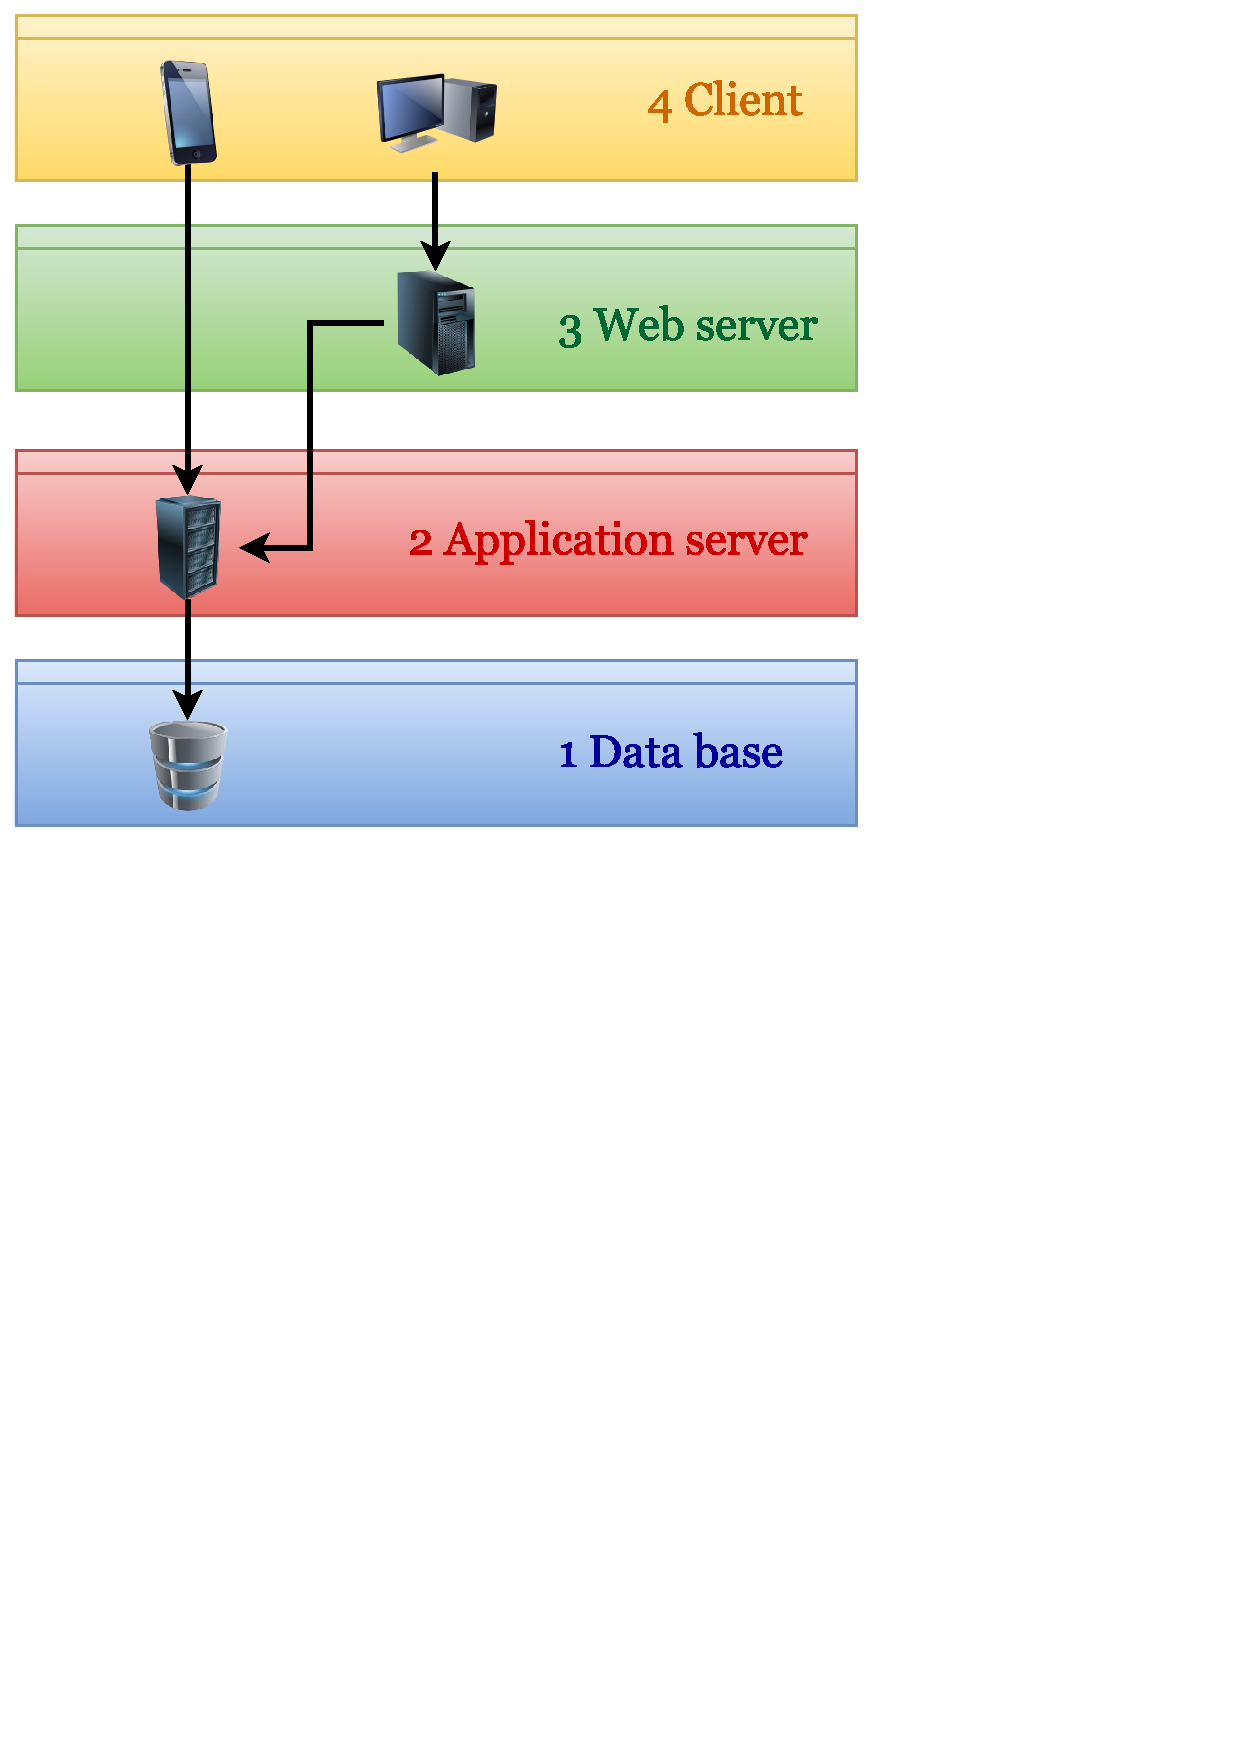
\includegraphics[width=0.7\textwidth]{diagrams/layers.pdf}
\caption{Layers of the system.}
\label{fig:layers}
\end{figure}

The interactions between the main components are shown in the figure \ref{fig:high_level_components}. They are all synchronous (obviously, the web server and the application server are multi-threaded).

\begin{figure}[h]
\centering
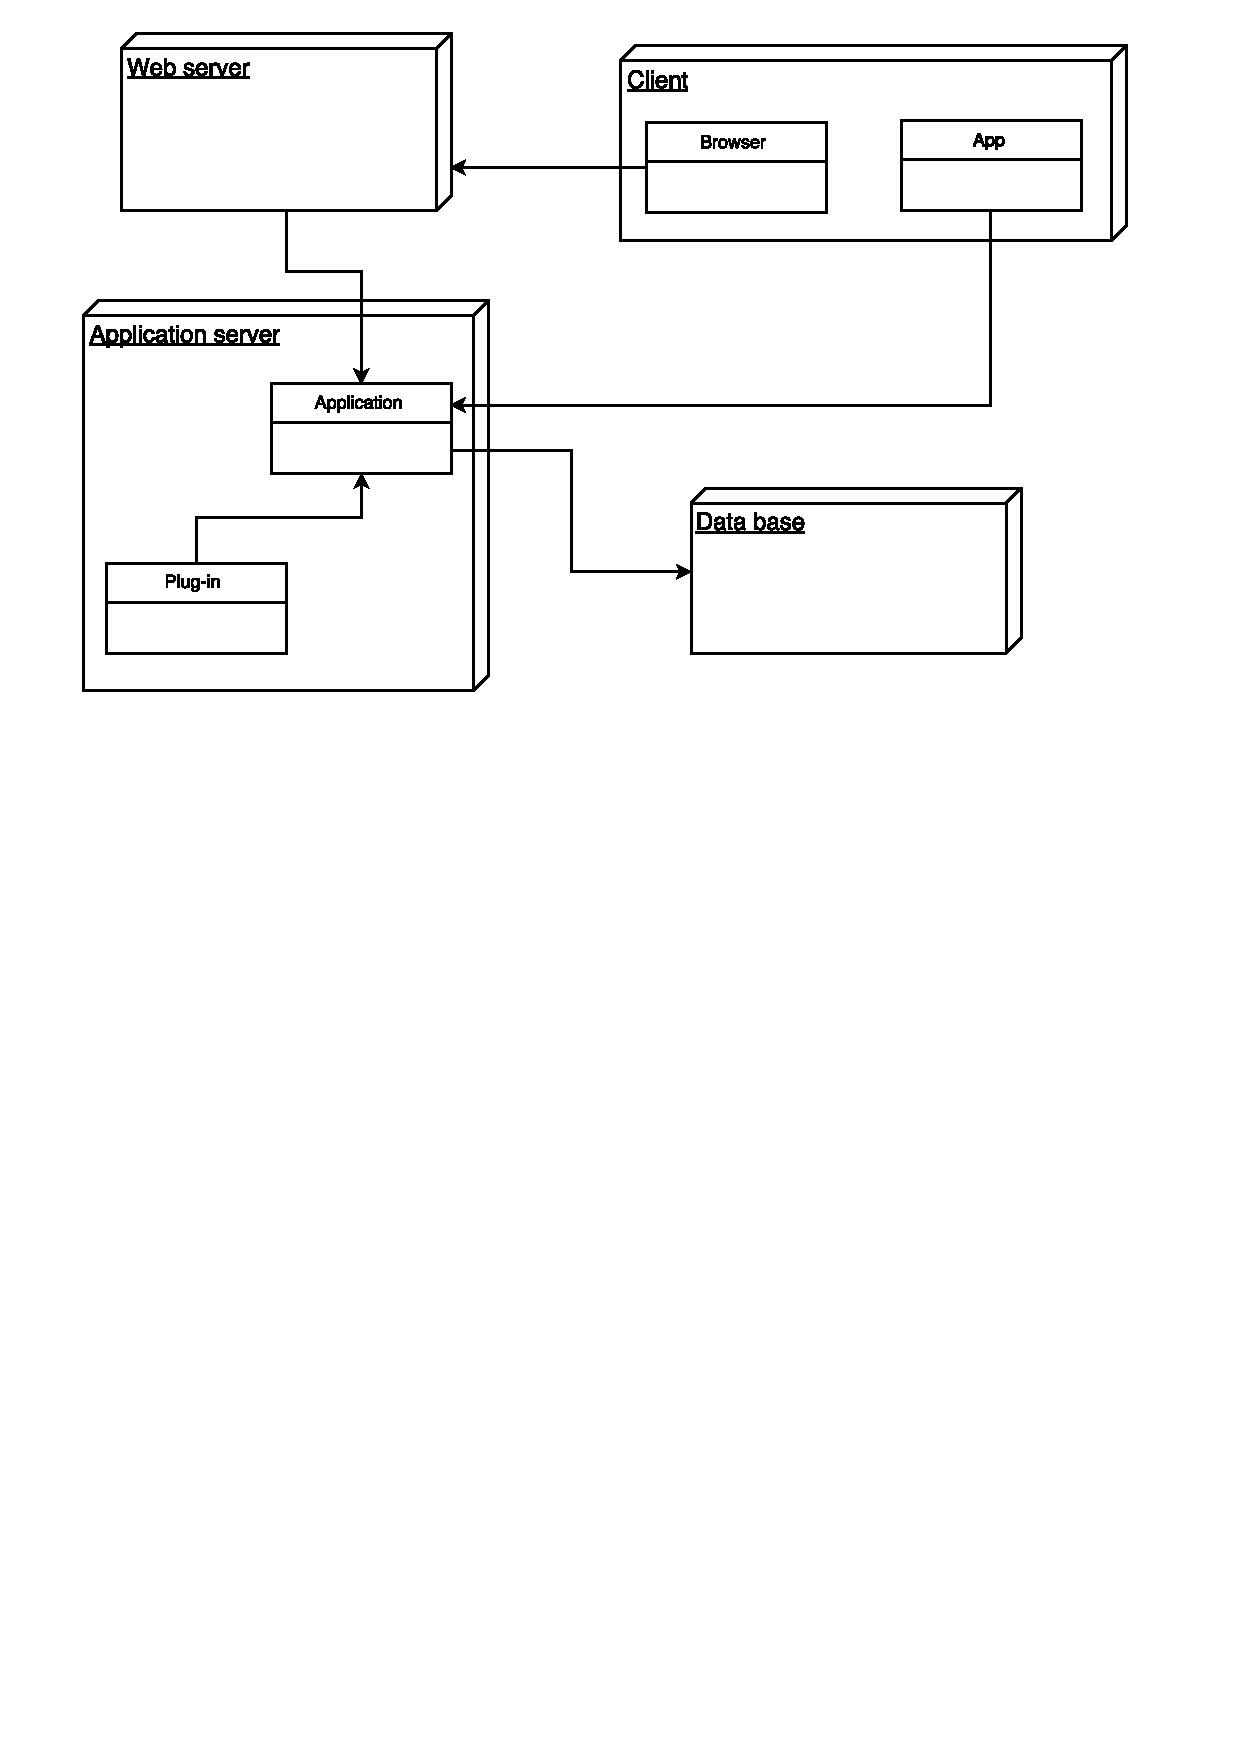
\includegraphics[width=\textwidth]{diagrams/high_level_components.pdf}
\caption{High level components of the system.}
\label{fig:high_level_components}
\end{figure}

\section{Component view}
\label{sec:component-view}

\begin{figure}
\centering
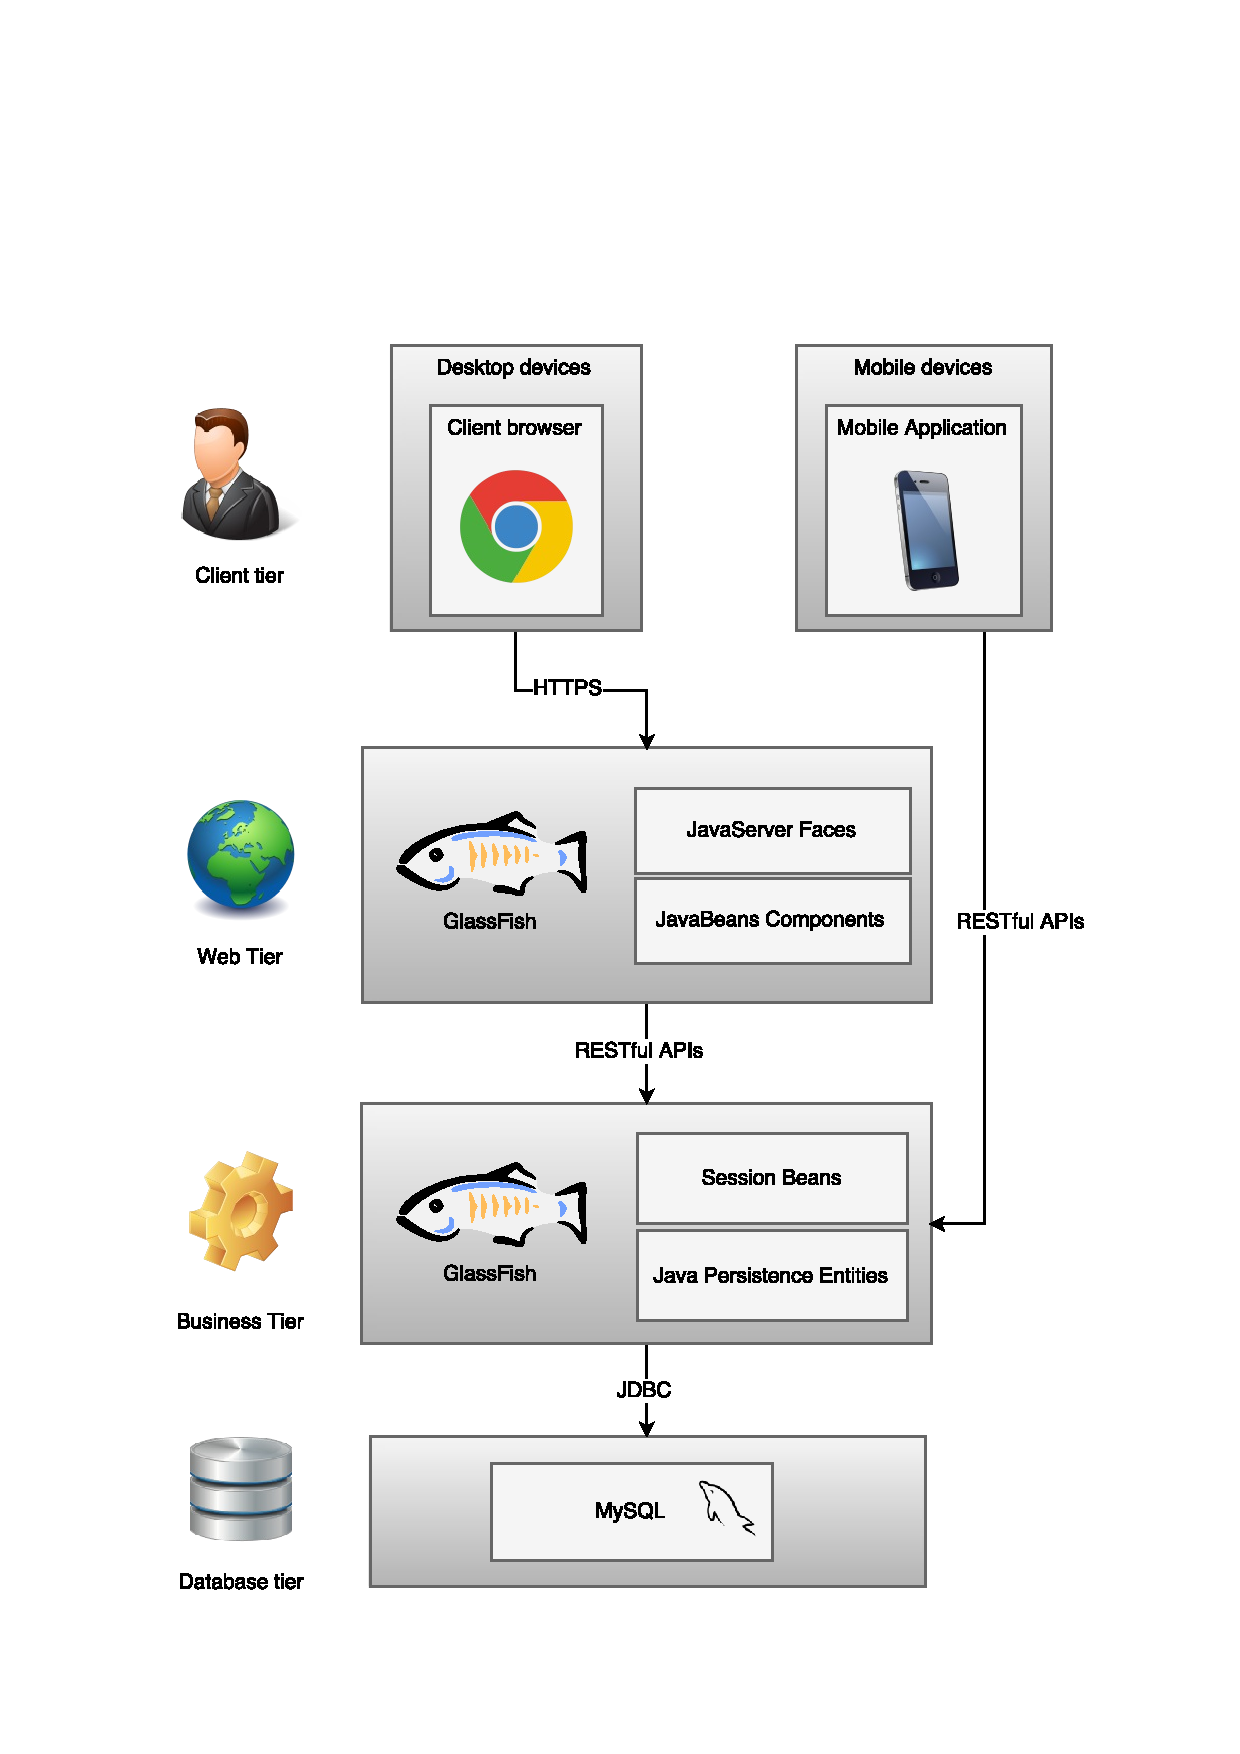
\includegraphics[width=\textwidth]{diagrams/JEE_Tiers}
\caption{The detailed description of tiers, detailed with JEE components.}
\label{fig:tiers-jee}
\end{figure}

\subsection{Database}
\label{sec:component-database}
The database tier runs MySQL Community Edition and uses InnoDB as the database engine: the DBMS has to support transactions and ensure ACID properties.
The DBMS will not be internally designed because it is an external component used as a ``black box'' offering some services: it only needs to be configured and tuned in the implementation phase.

The database can communicate only with the business logic tier using the standard network interface, described in \autoref{sec:component-interfaces}.
Security restrictions will be implemented to protect the data from unauthorized access: the database must be physically protected and the communication has to be encrypted. Access to the data must be granted only to authorized users possessing the right credentials. Every software component that needs to access the DBMS must do so with the minimum level of privilege needed to perform the operations.

All the persistent application data is stored in the database. The conceptual design of the database is illustrated by the E-R diagram in~\autoref{fig:er-diagram}.

\begin{figure}
    \centering
    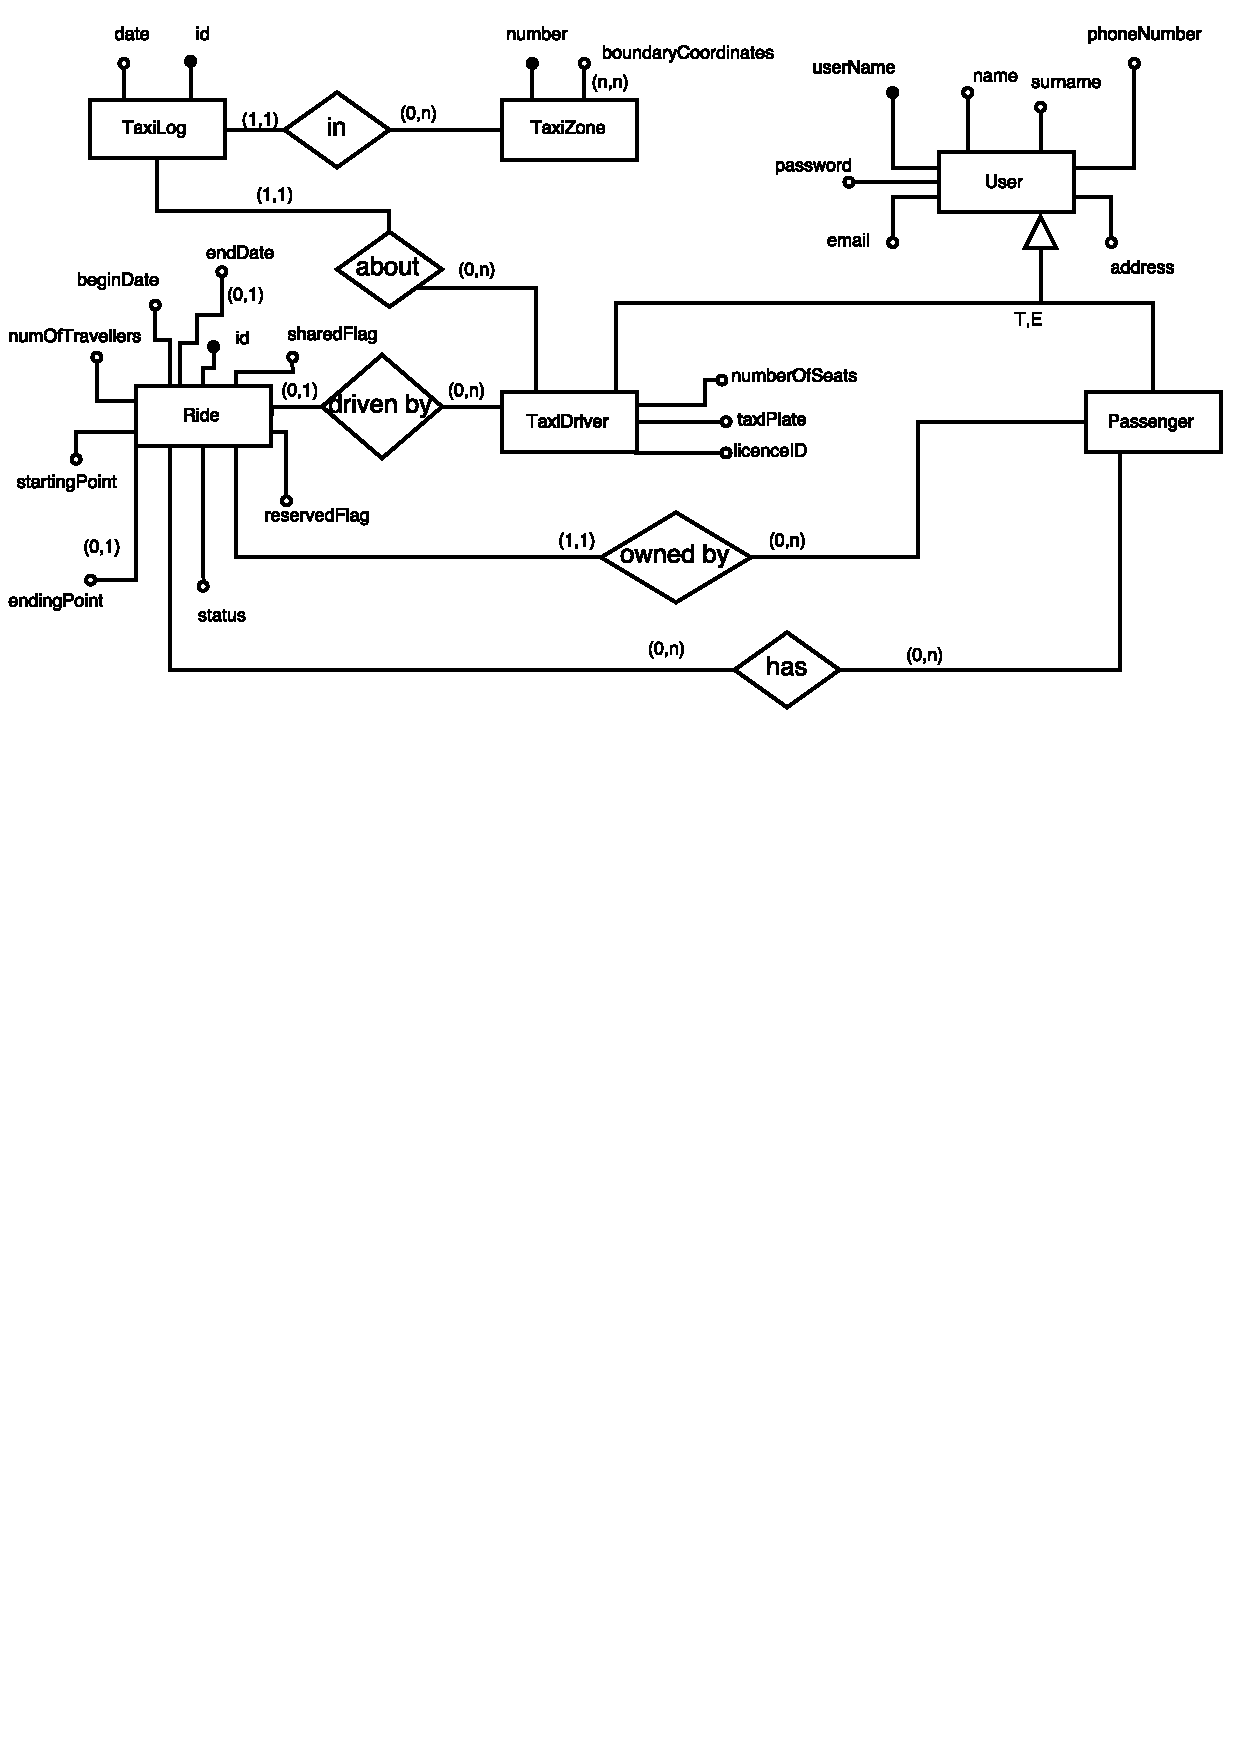
\includegraphics[width=\textwidth]{diagrams/er_diagram}
    \caption{The Entity-Relationship diagram of the database schema.}
    \label{fig:er-diagram}
\end{figure}

Foreign key constraints and triggers are not used: the dynamic behaviour of the data is handled entirely by the Java Persistence API in the Business Application tier.

\subsection{Application server}
The application server is implemented in the business logic tier using Java EE; it runs on GlassFish Server.

The access to the DBMS is not implemented with direct SQL queries: instead, it is completely wrapped by the \textbf{Java Persistence API (JPA)}. The object-relation mapping is done by entity beans.

The Entity Beans representing the database entities (\autoref{fig:entity-diagram}) are strictly related to the entities of the ER diagram (\autoref{fig:er-diagram}).

\begin{figure}
    \centering
    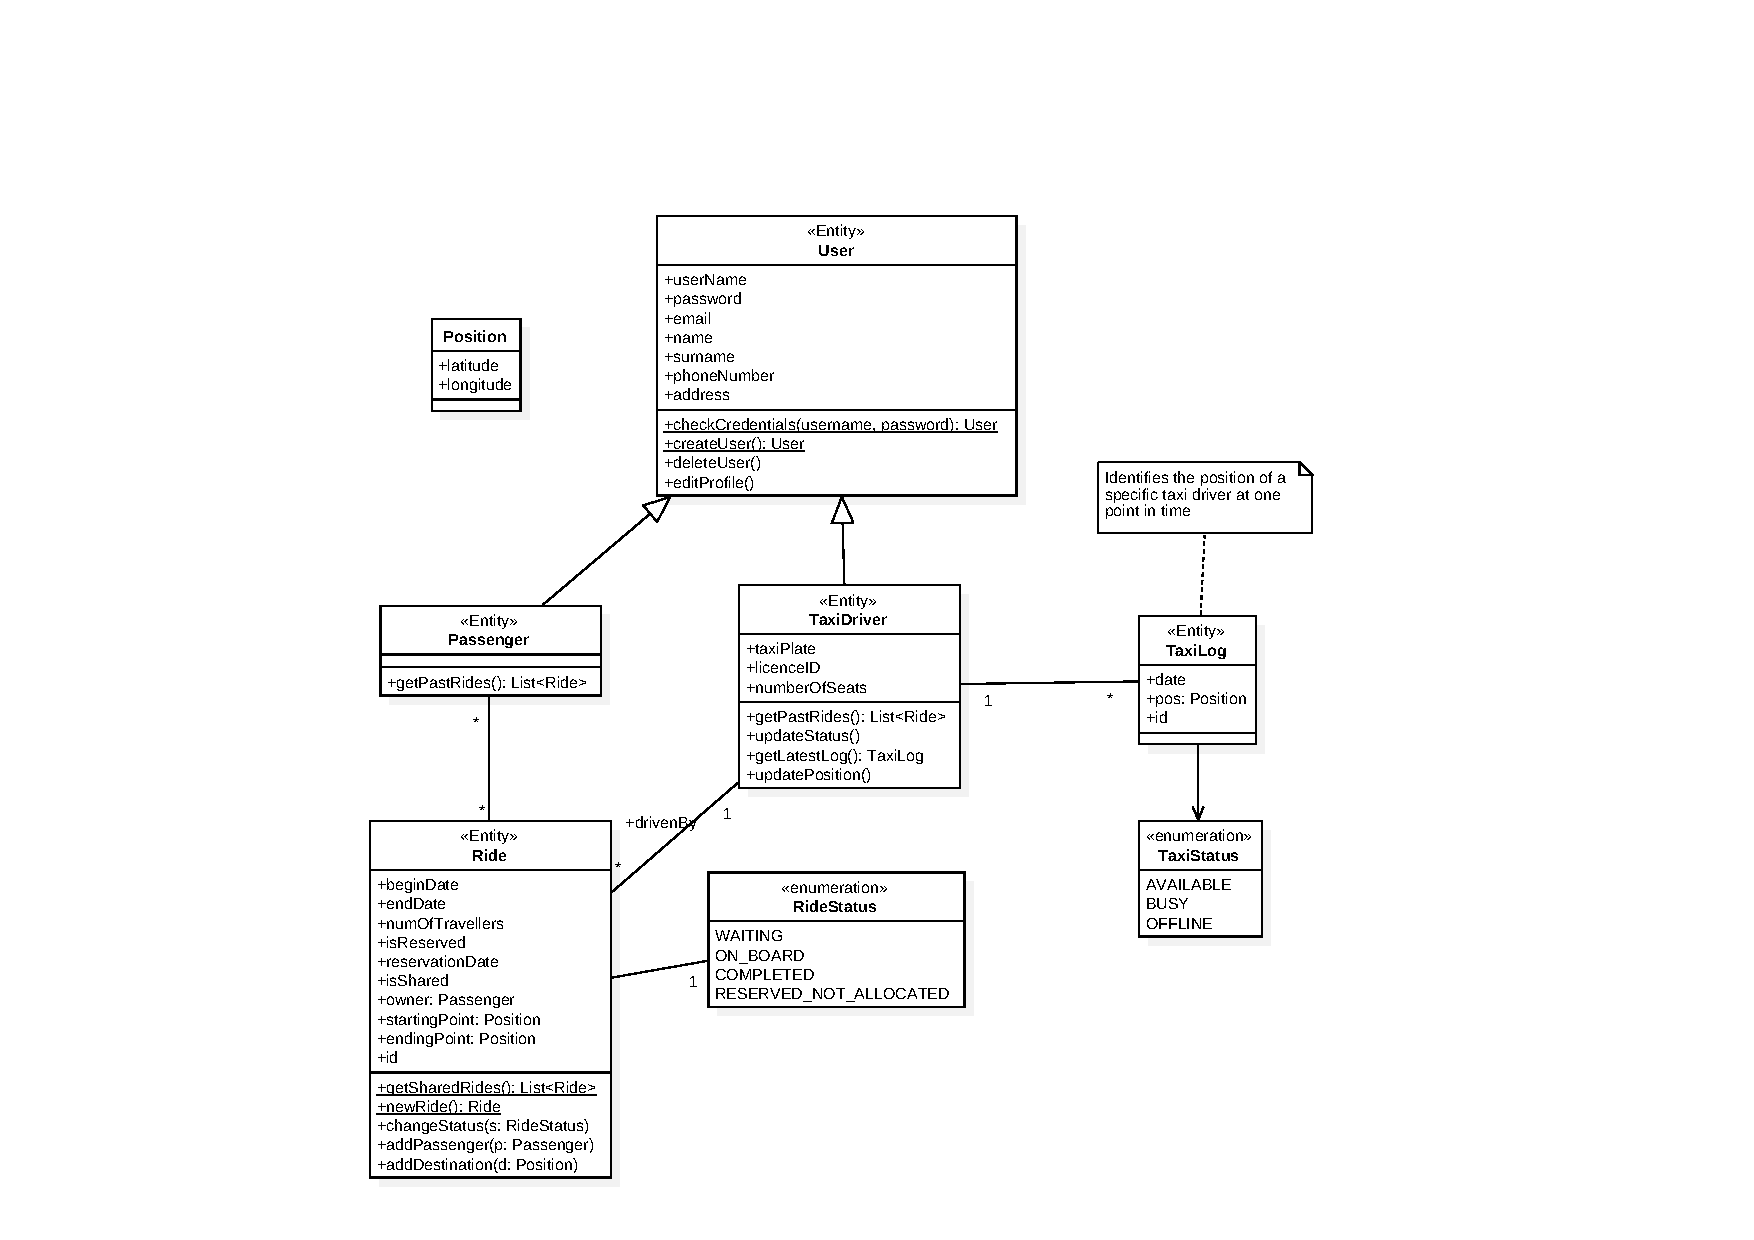
\includegraphics[width=\textwidth]{diagrams/entity_diagram}
    \caption{Java Entity Beans used to represent the entities in the database.}
    \label{fig:entity-diagram}
\end{figure}

The business logic is implemented by custom-built \textbf{stateless Enterprise JavaBeans (EJB)}.
Our application indeed is rather simple and message-driven: the state of the users is stored in the DB, so we do not generally need stateful EJBs which can be more expensive.
Concurrency management and performance are fundamental, so the reusal of EJBs for many request is a desirable behaviour.

The application server implements a RESTful API using JAX-RS to allow the clients (web tier and mobile client) to use the services offered by the EJBs: this interface will be thoroughly discussed in~\autoref{sec:rest-api}.

Session Beans used for the application server are shown in~\autoref{fig:session-beans}.

\subsubsection{UserManager}
This bean manages all the user management features, namely: user login, user registration, user deletion, user profile editing.
It also provides a function to confirm the email address provided by the user with the token sent by email.

\subsubsection{RideManager}
This bean creates new rides, assigns passengers and taxi driver to existing rides and fetches information about rides.
It also allows taxi drivers to update the status of a ride, signaling when the passengers are on board and when the ride is finished.

\subsubsection{TaxiManager}
This bean handles the availability status and the position of each taxi driver.
Taxi drivers can mark themselves as available or unavailable, and they can change their position as well.
This component also has a method to find the first taxi in the queue for a specific taxi zone.

This component is stateless and can be instantiated multiple times. It calls TaxiQueueManager for data access.

\subsubsection{TaxiQueueManager}
This bean is a singleton and is in charge of keeping track of the taxi queue for each taxi zone.
Taxi queues are not persistent data, so they are not stored in the database: they are only present in main memory.
This allows a quicker access since this data is changed often.

The TaxiQueueManager keeps references to TaxiQueues and updates them when a taxi driver changes his status or his position.
This component also has a method to find the first taxi in the queue for a specific taxi zone.

This component takes responsibility to ensure a correct concurrent access to the queues.

\subsubsection{HistoryManager}
This bean allows users (passengers and taxi drivers) to fetch the history of their past rides.
This component is accessed by the RideManager and is able to store the rides which have ended.

\subsubsection{EmailSender}
This bean is in charge of sending emails to users when needed.
For now its only functionality is to send the e-mail confirmation token to the user e-mail address after the registration, but in future implementations it could be extended to implement e-mail notifications.

\subsubsection{SharedRidePlugin}
This plugin implements all the functions related to the taxi sharing feature.
It allows the passengers to find feasible shared rides and join them.

\subsubsection{ReservedRidePlugin}
This plugin implements all the functions related to the ride reservation feature.
This component allows passengers to reserve a taxi for a future time.

\subsubsection{ConfiguratorBean}
This bean is a singleton and its only duty is to read the server configuration file and provide the value of configuration options to other components.
Settings are stored as a set of key-value pairs.
Other beans can ask for configuration options using the same keys used to define the settings in the configuration file.

\begin{figure}
    \centering
    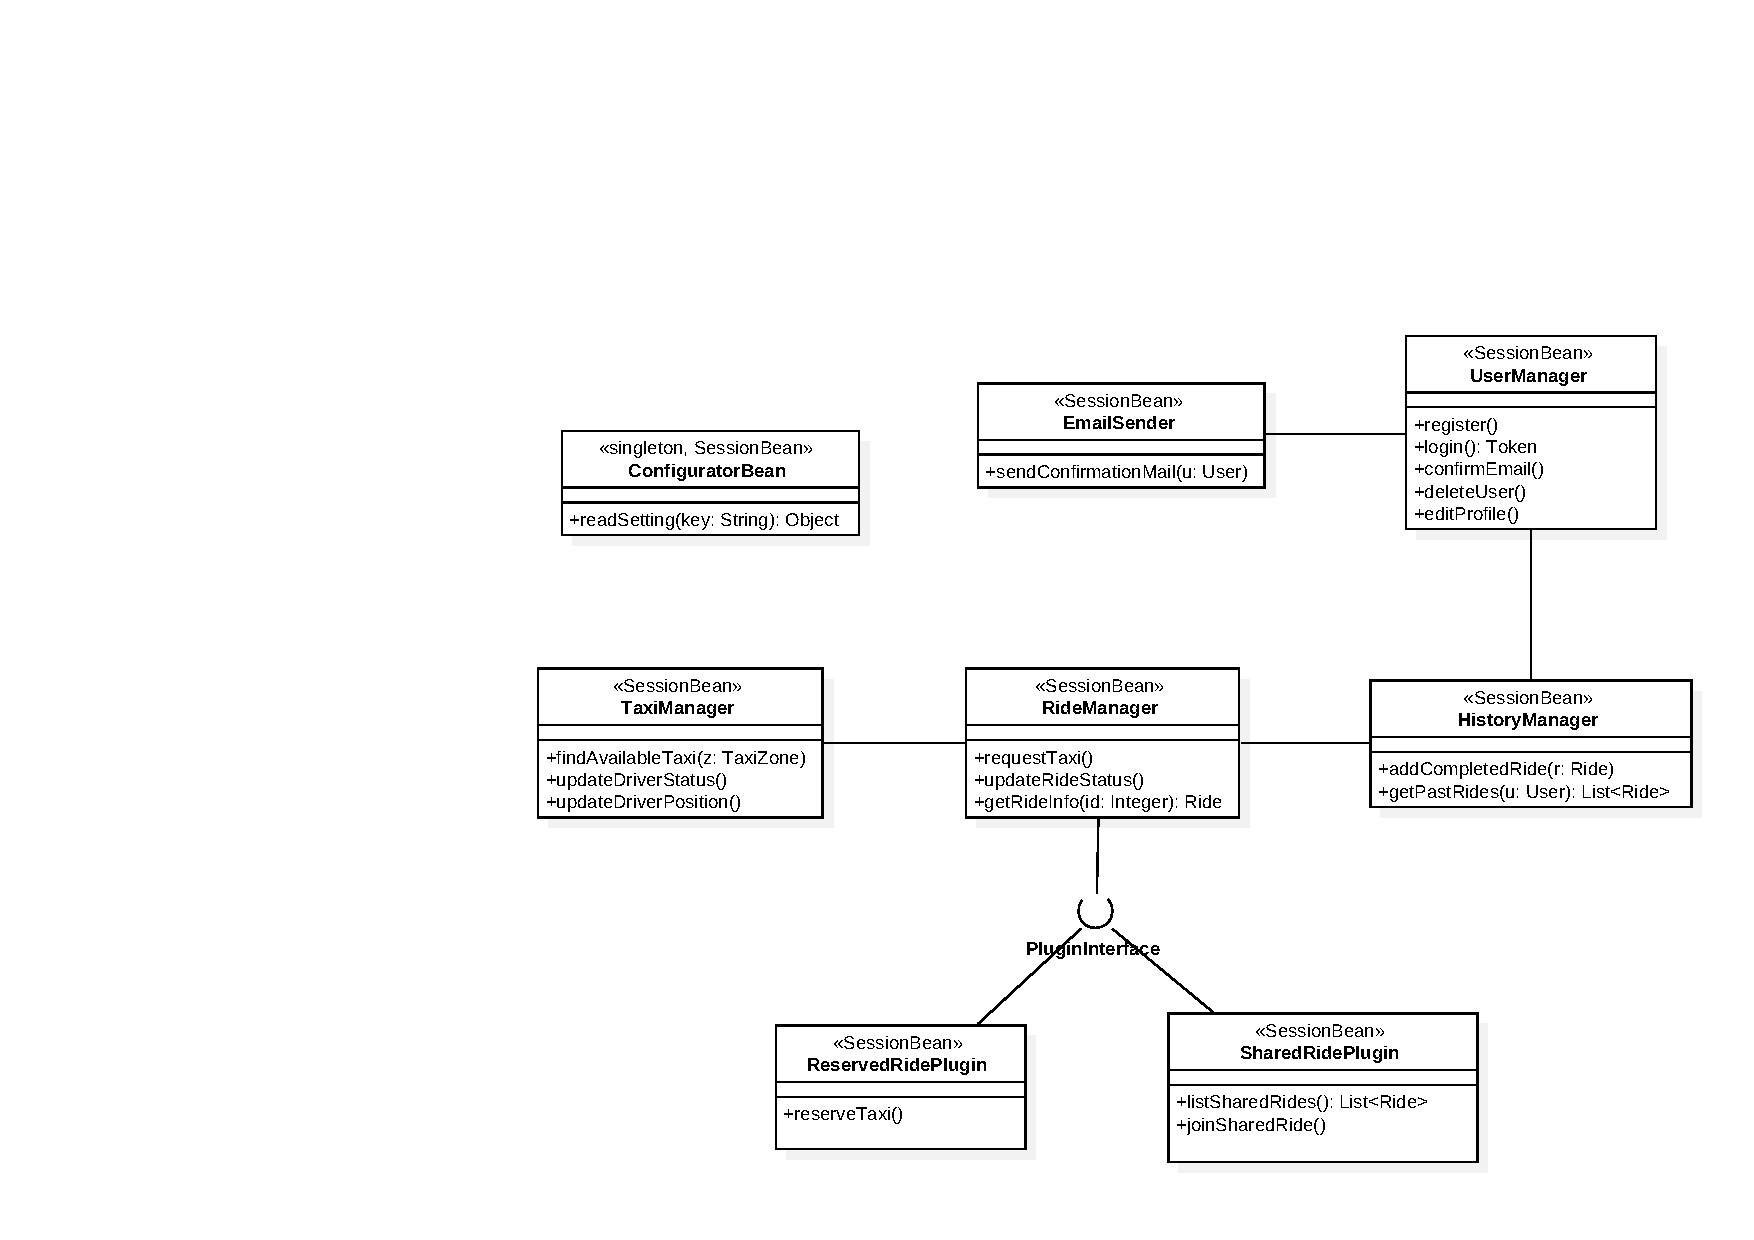
\includegraphics[width=\textwidth]{diagrams/class_sessionbeans}
    \caption{The session beans used in the implementation of the business logic. The parameters of the methods are not written here: the detailed interface of each bean is described in detail in~\autoref{sec:rest-api}}.
    \label{fig:session-beans}
\end{figure}

\subsection{Web server}
\label{sec:comp-view-web-server}
The web server is implemented using Java EE web components, namely JavaServer Faces (JSF), which is a server-side framework based on MVC.
The web server is run by GlassFish Server.

The web tier only implements the presentation layer: all the business logic is handled by the application server tier. The web tier uses the RESTful interface of the application tier.

Using JSF, the view is written as XML files and is completely separated from the logic of the web server. This enables us to write a modular web service.

The web server architecture is composed simply by JSF (as the view) and by a controller class that takes the user input and translates it in API requests (\autoref{fig:web-components}).

\begin{figure}
    \centering
    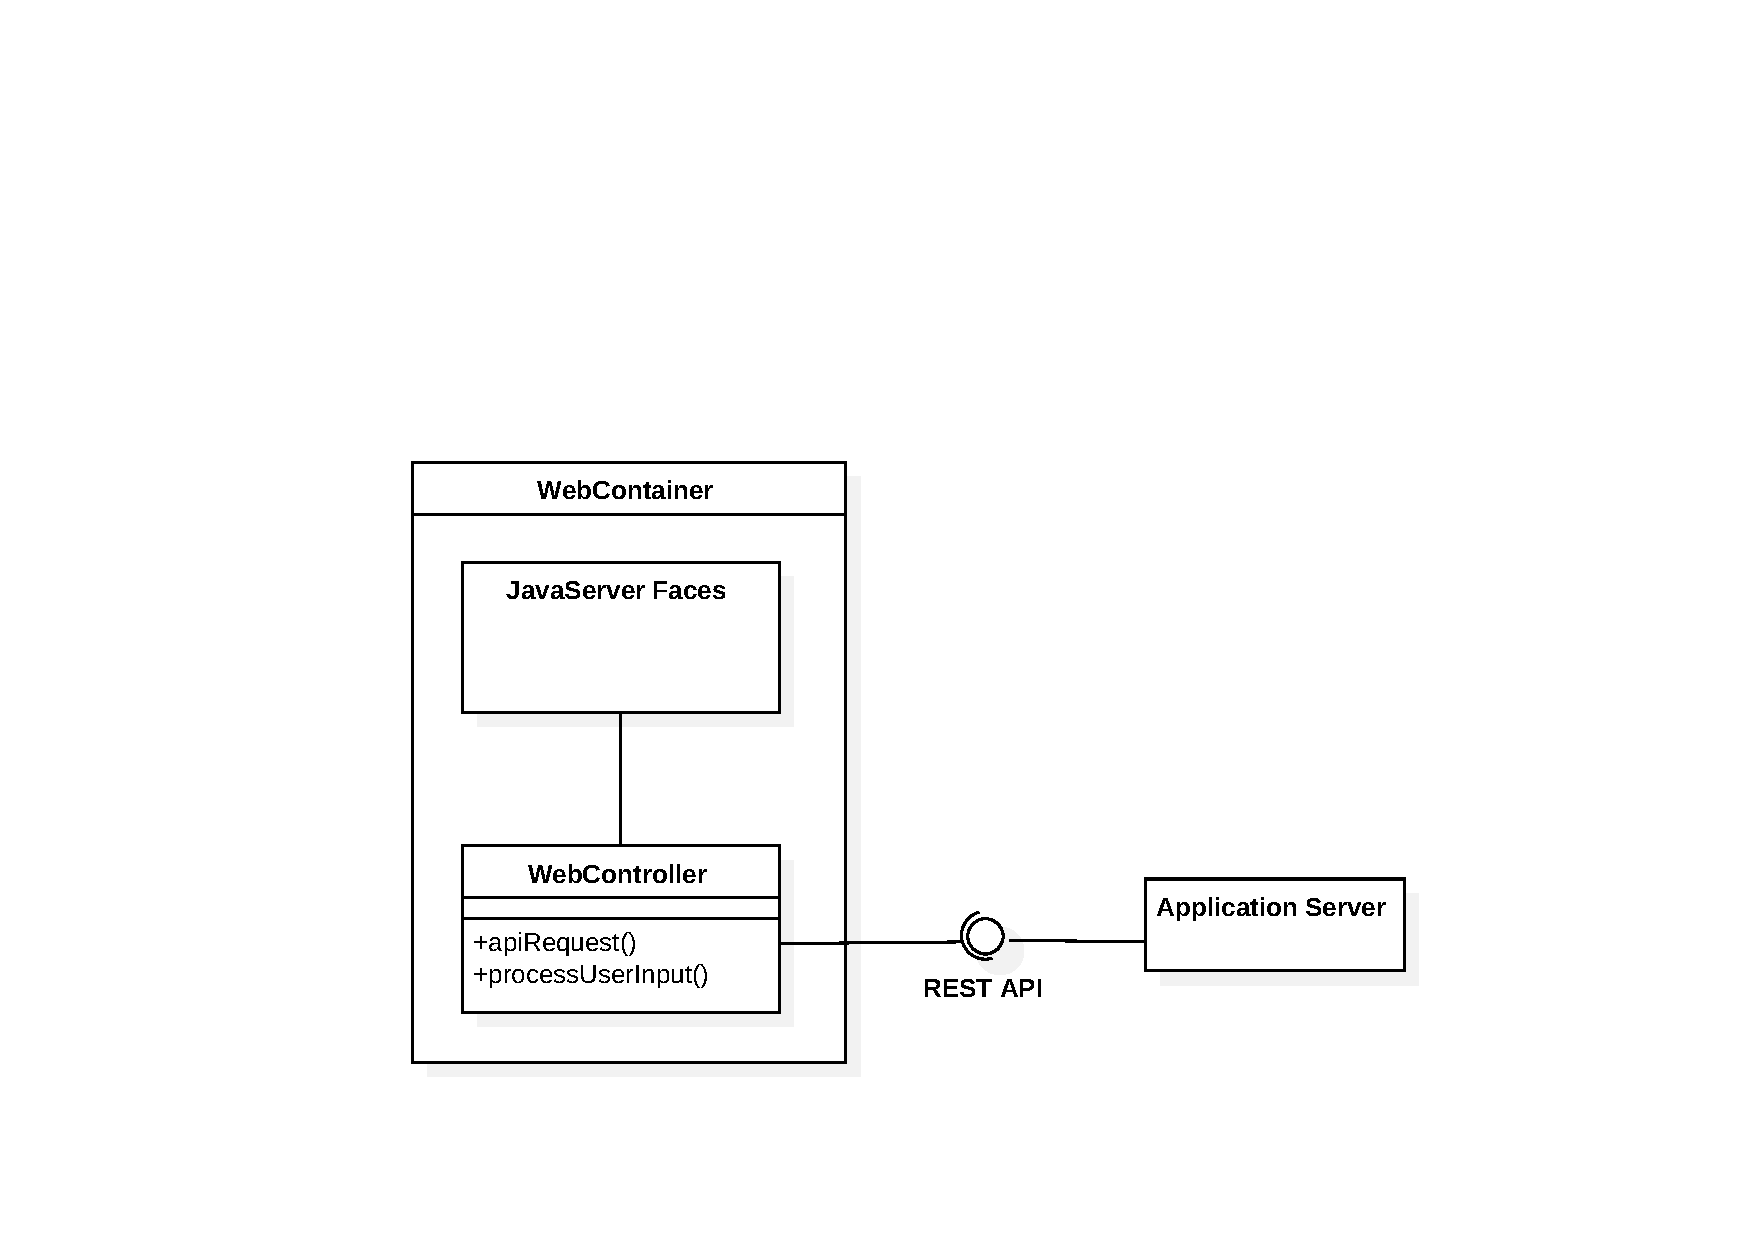
\includegraphics[width=\textwidth]{diagrams/class_webcomponents}
    \caption{The components of the web tier.}
    \label{fig:web-components}
\end{figure}

\subsection{Mobile client}
The mobile client implementation depends on the specific platform. 
The iOS application is implemented in Swift and mainly uses \textbf{UIKit} framework to manage the UI interface.
Instead, the Android application is implemented in Java and mainly uses \textbf{android.view} package for graphical management.

The application core is composed by a controller which translates the inputs from the UI into remote functions calls via  RESTful APIs. The controller also manages the interaction with the GPS component using  \textbf{CoreLocation} framework in iOS app and \textbf{LocationListener} interface in the Android one.

The main structure of the mobile application is shown in figure \autoref{fig:mobile-app}.

\begin{figure}
    \centering
    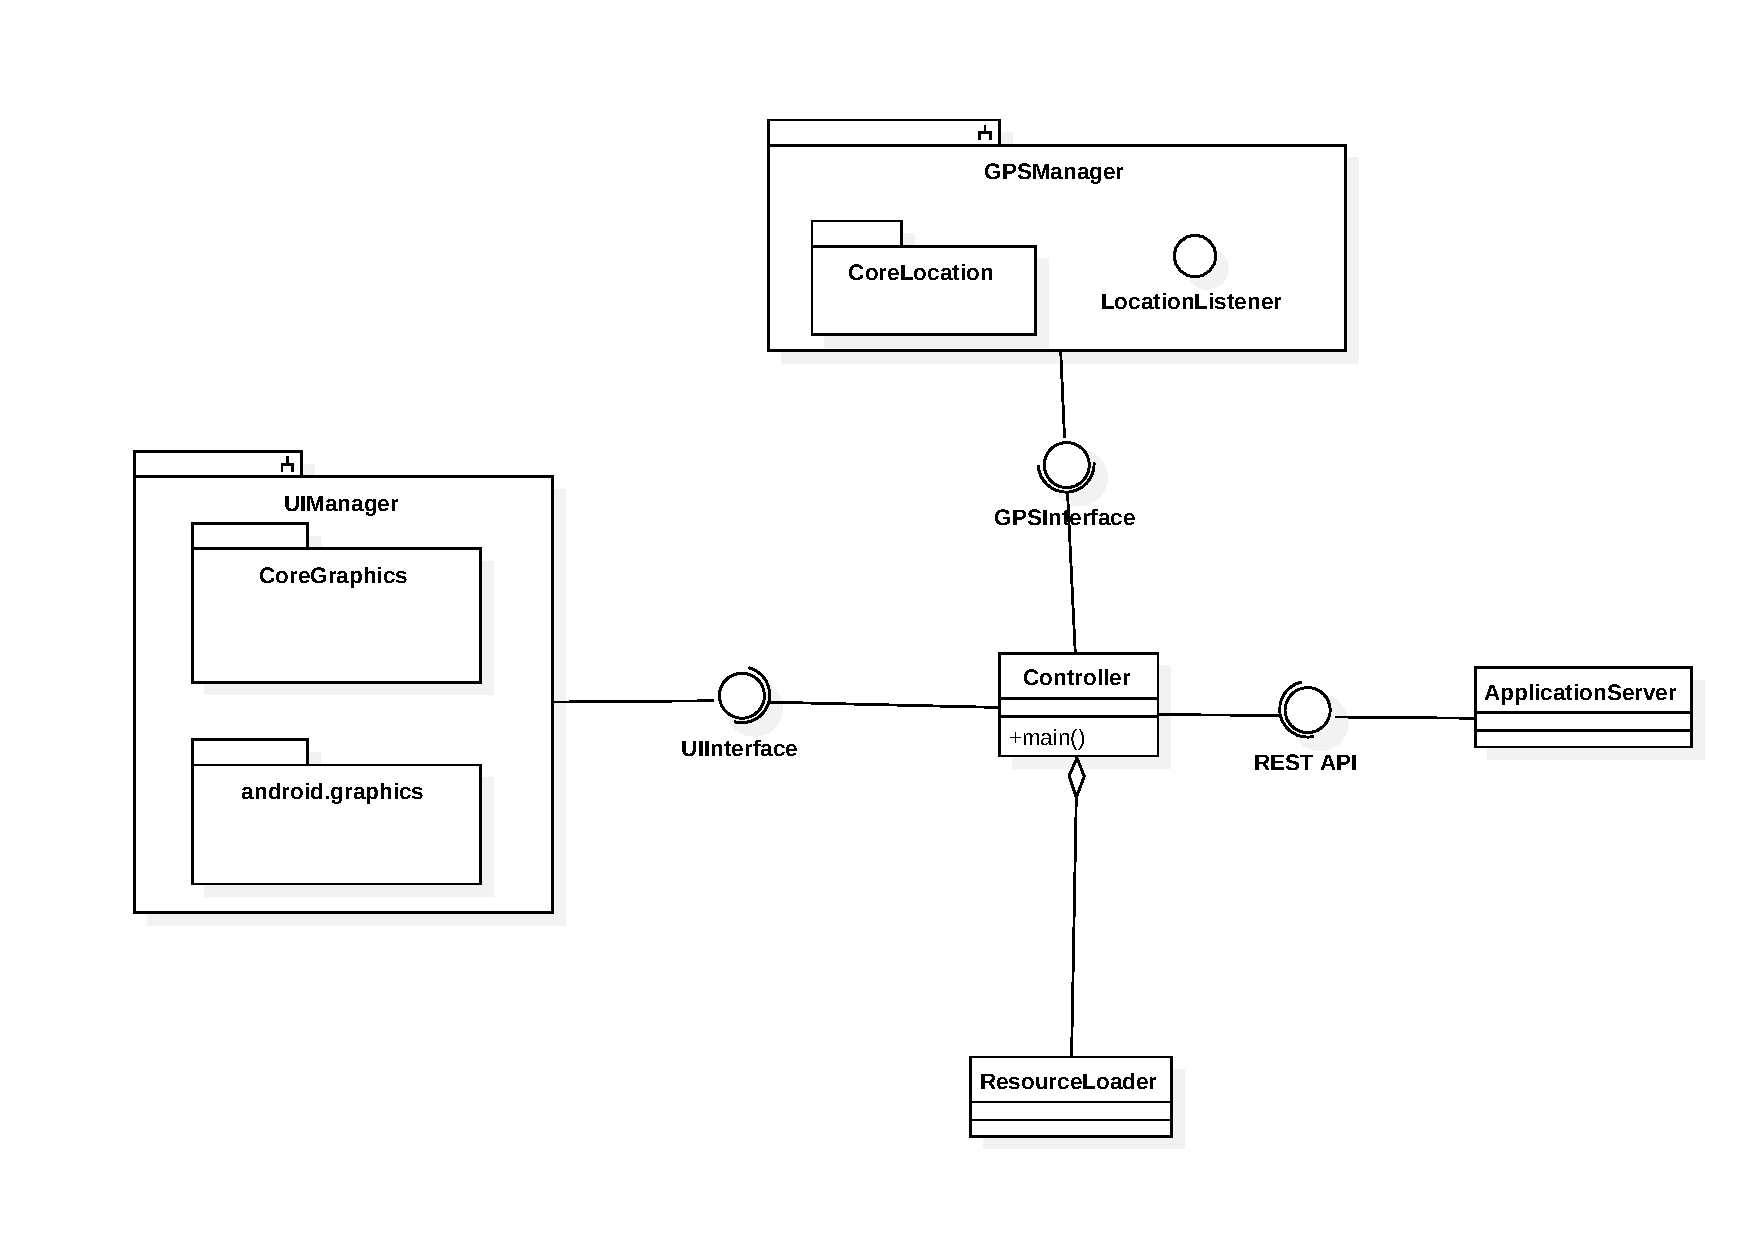
\includegraphics[width=\textwidth]{diagrams/class_mobileapp}
    \caption{The components of the mobile app.}
    \label{fig:mobile-app}
\end{figure}


\FloatBarrier

\section{Deployment view}
\label{sec:deployment-view}

The deployment diagram for the system is shown in~\autoref{fig:deployment-diagram}.
\begin{figure}[h]
\centering
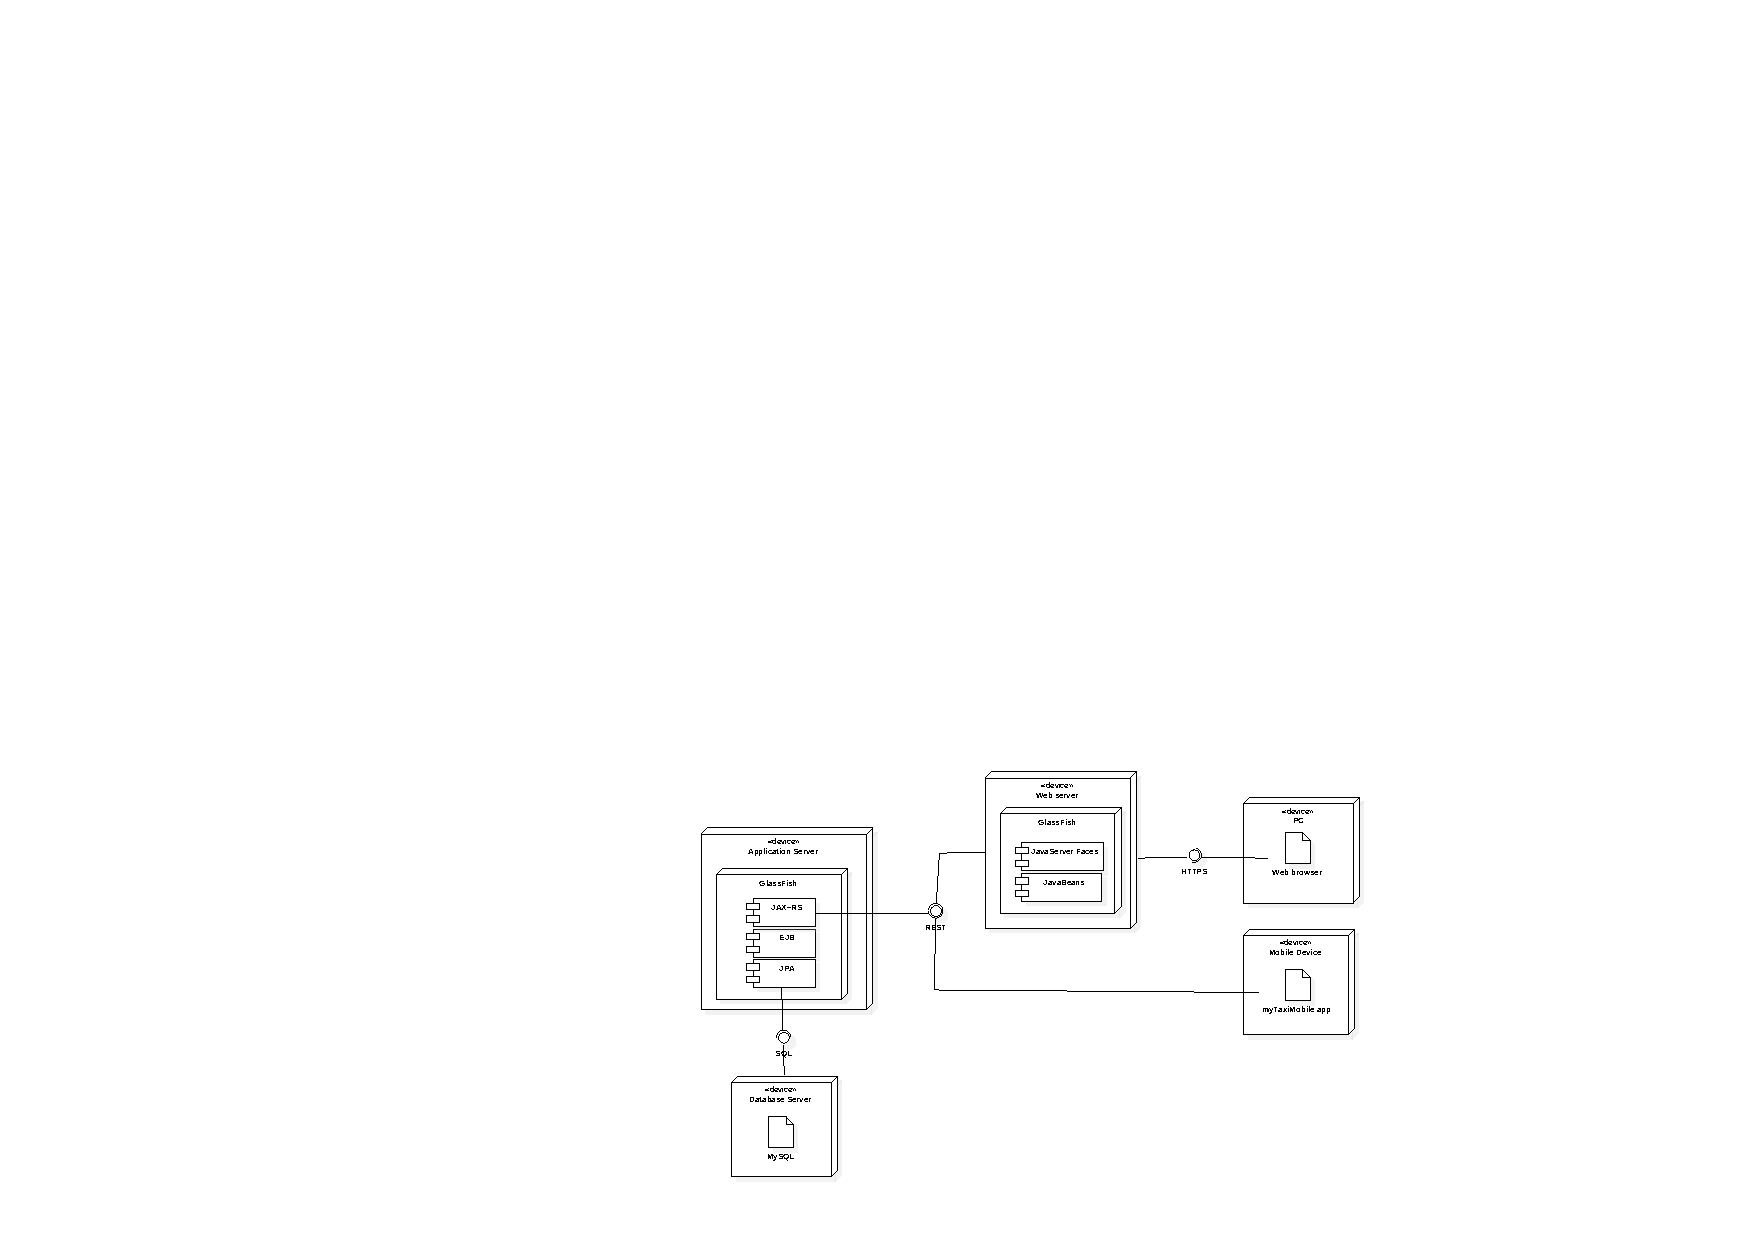
\includegraphics[width=\textwidth]{diagrams/deployment_diagram}
\caption{The deployment diagram for our application.}
\label{fig:deployment-diagram}
\end{figure}

\section{Runtime view}
\label{sec:runtime-view}

In this section we will describe the dynamic behaviour of the system.
In particular, it will be shown how the software and logical components defined in \autoref{sec:component-view} interact one with another, using \emph{sequence diagrams} for the more meaningful functionalities of the system.

Also, \emph{runtime unit diagrams} will be shown in some use cases of the software: these diagrams show the instances of the components running in the tiers when the users interact with the system.

\begin{figure}[h]
    \centering
    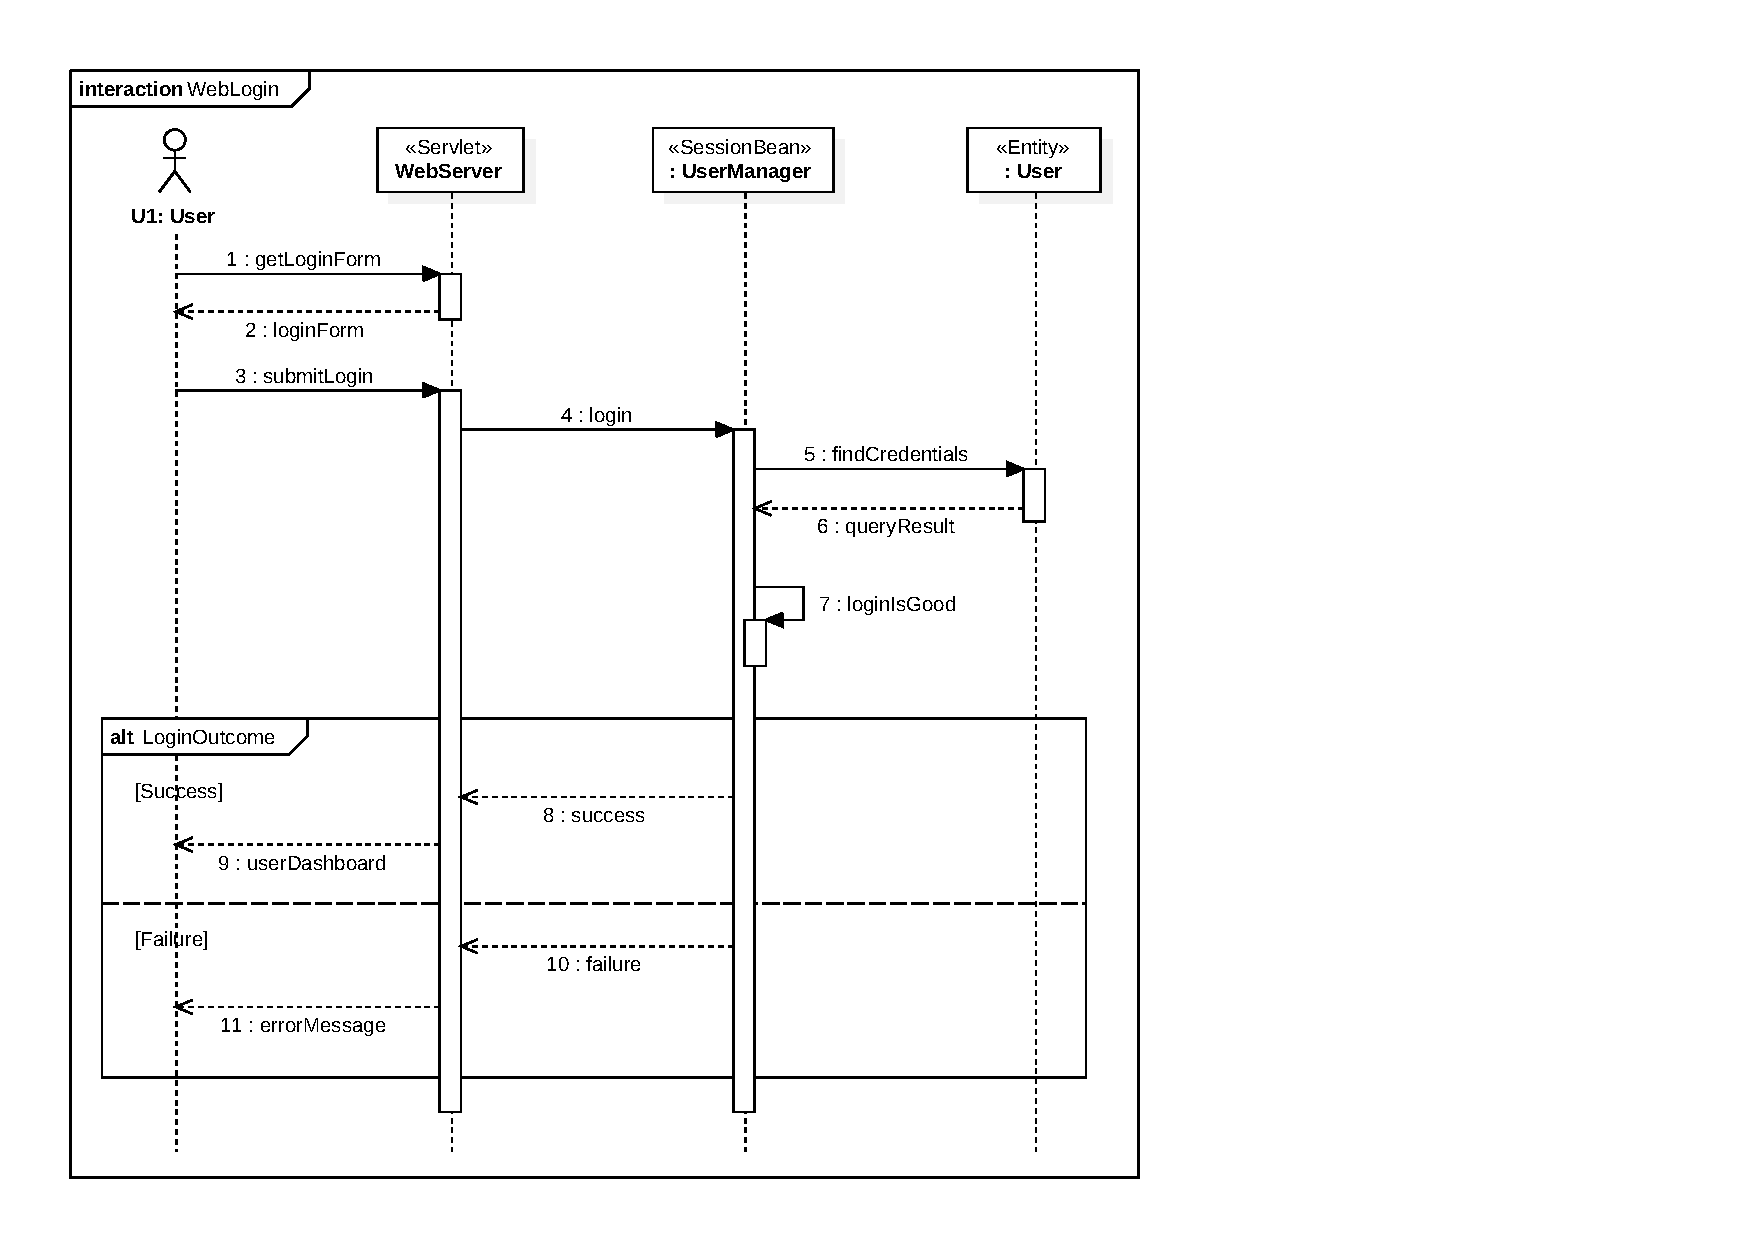
\includegraphics[width=\textwidth]{diagrams/sequence_weblogin}
    \caption{Sequence diagram of the login with the web interface.}
    \label{fig:sequence-weblogin}
\end{figure}

\begin{figure}[h]
    \centering
    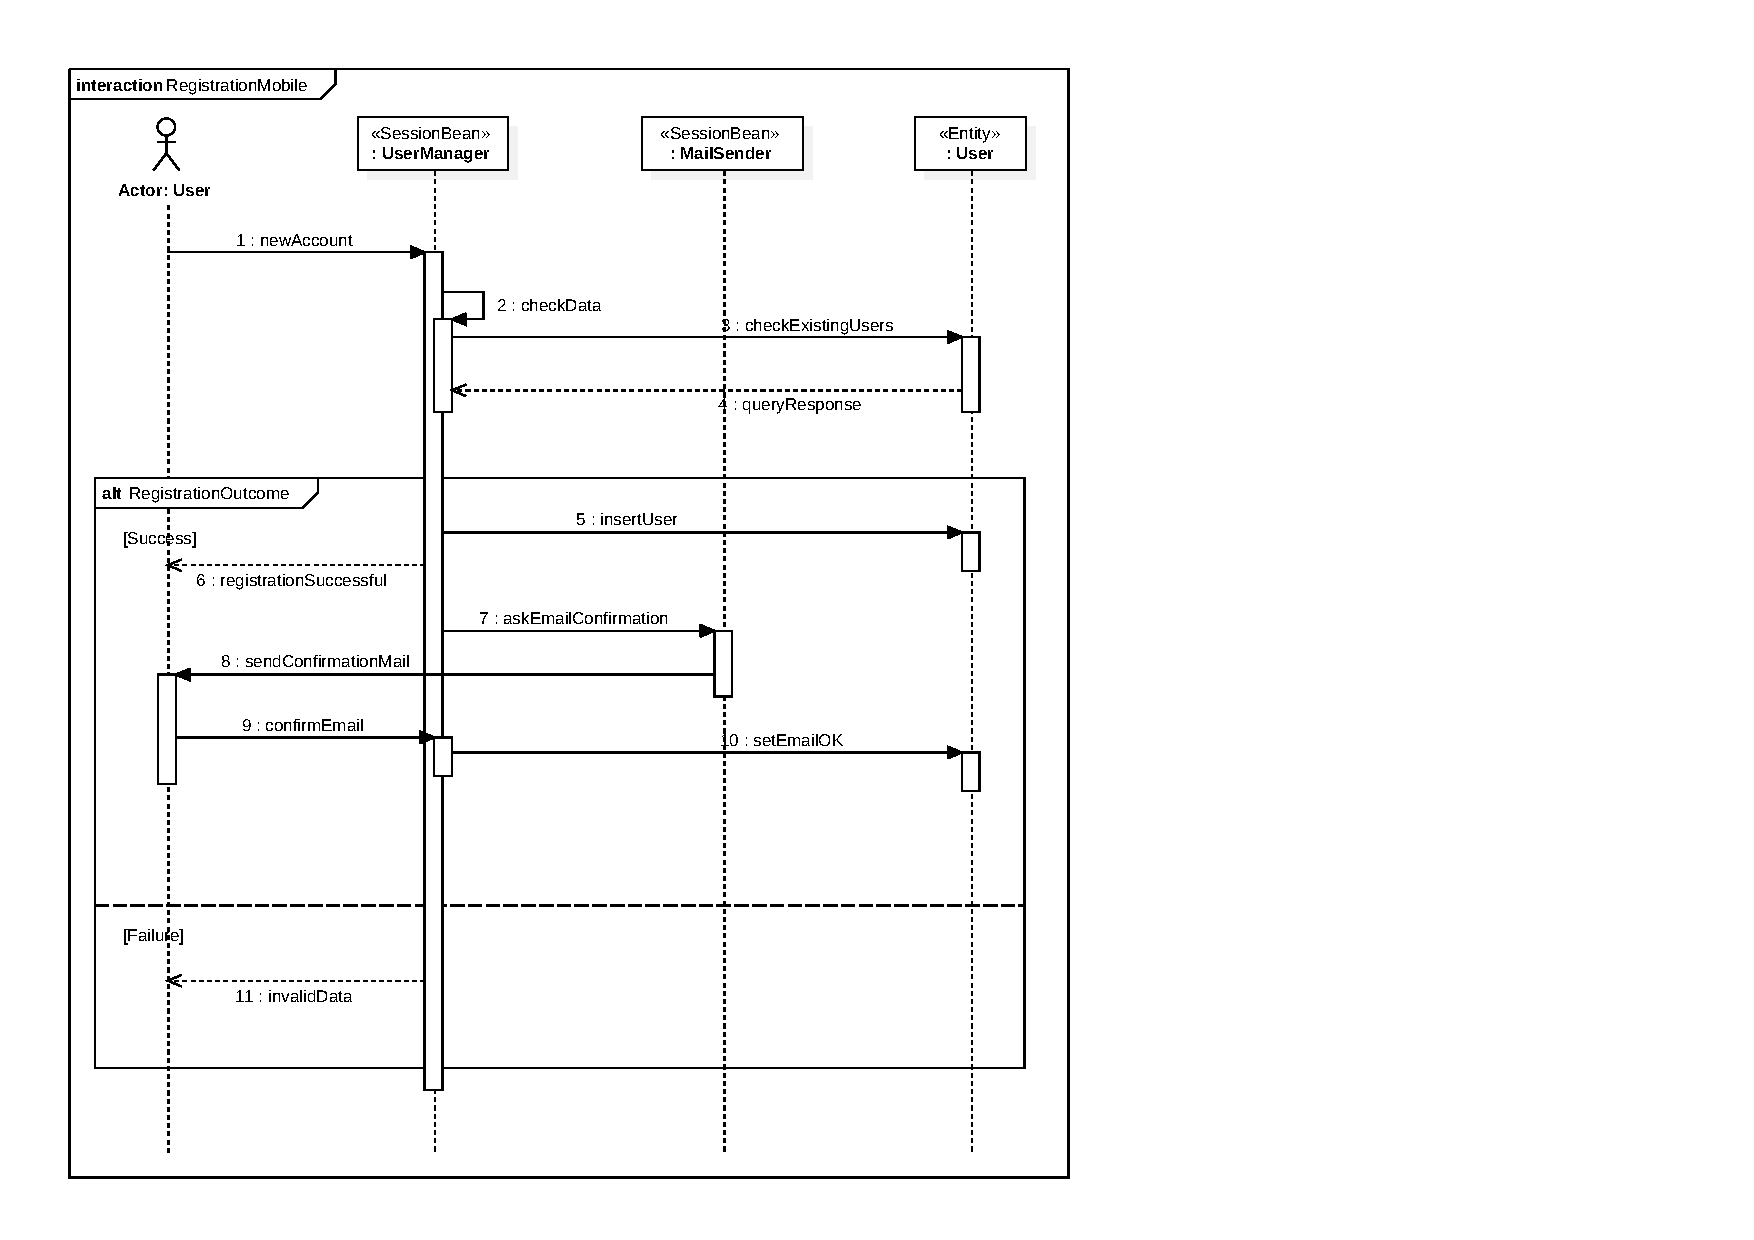
\includegraphics[width=\textwidth]{diagrams/sequence_registrationmobile}
    \caption{Sequence diagram of the registration from a mobile client.}
    \label{fig:sequence-registrationmobile}
\end{figure}

\begin{figure}[h]
    \centering
    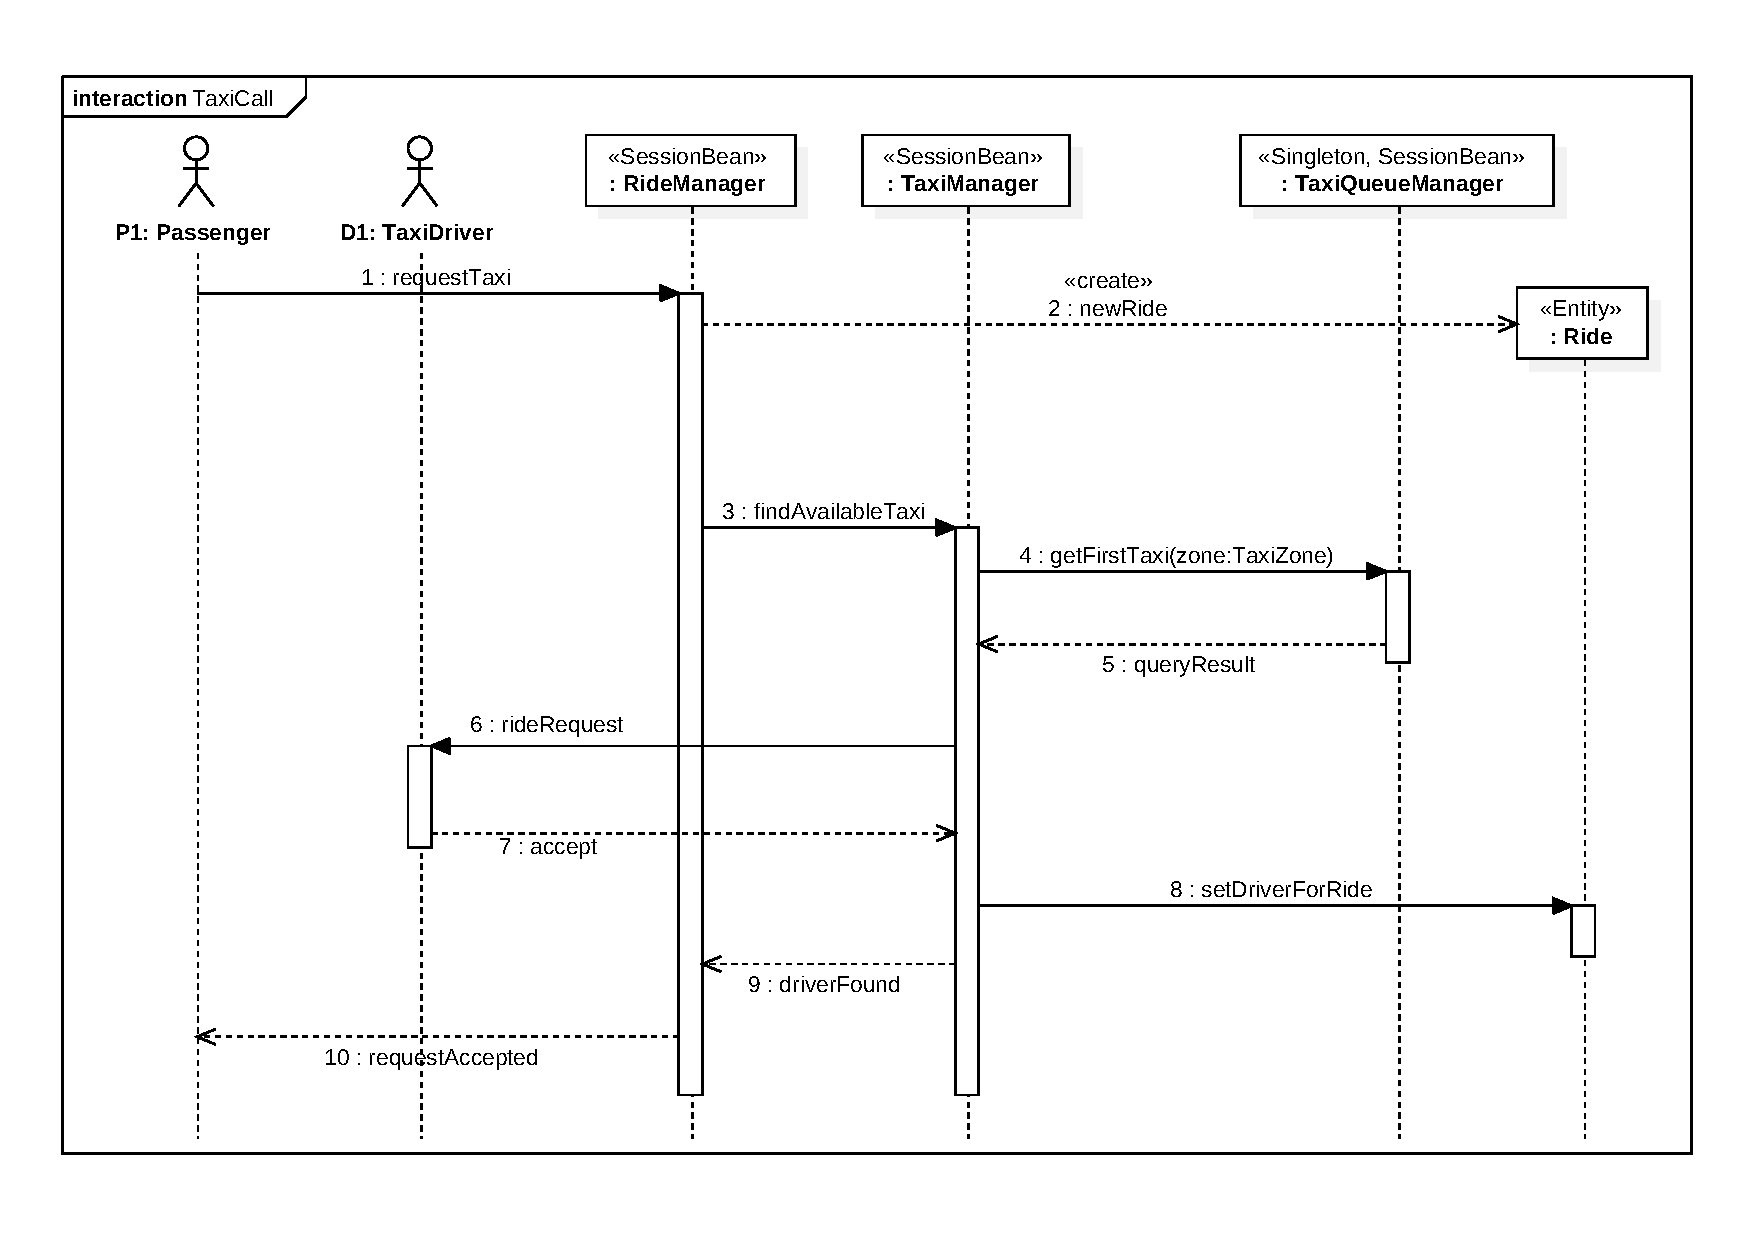
\includegraphics[width=0.8\textwidth]{diagrams/sequence_taxicall}
    \caption{Sequence diagram of a taxi call.}
    \label{fig:sequence-taxicall}
\end{figure}

\begin{figure}[h]
    \centering
    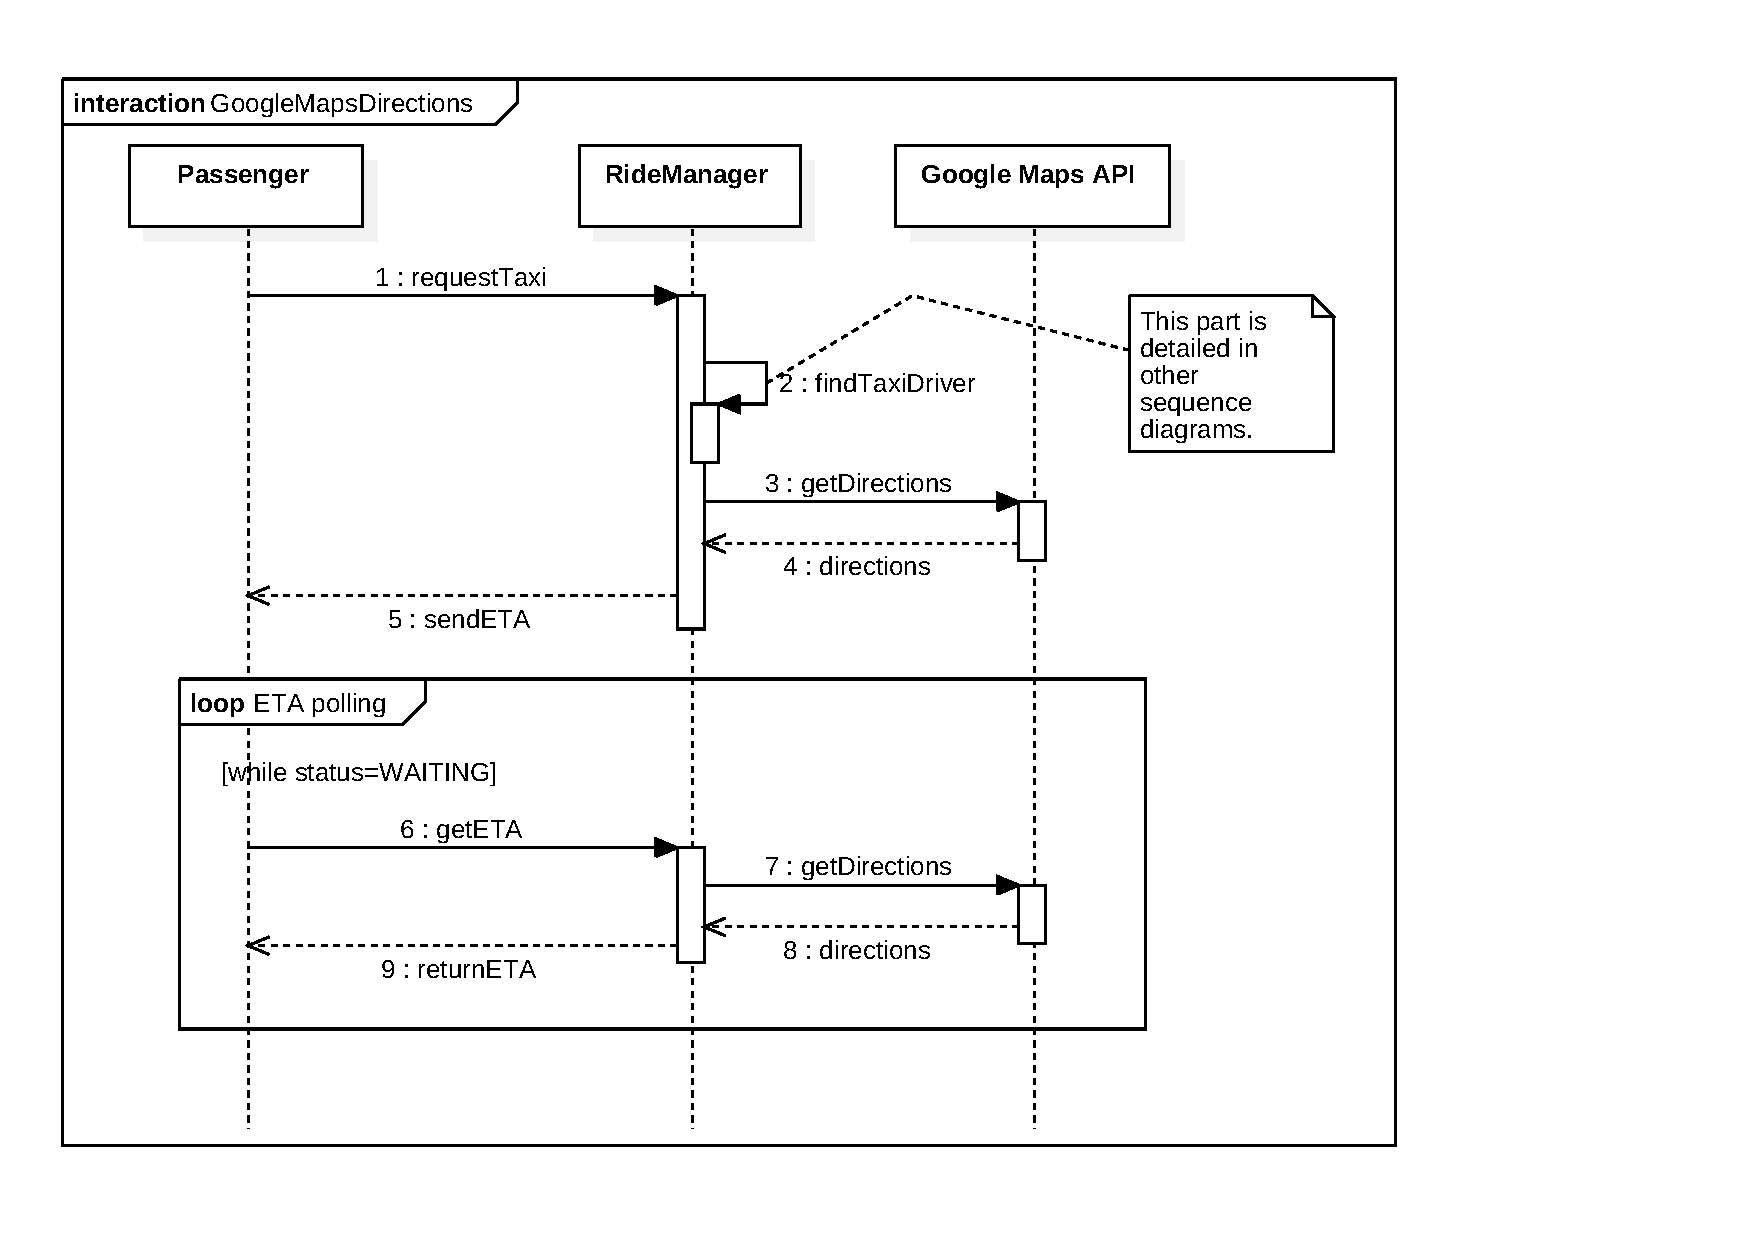
\includegraphics[width=0.8\textwidth]{diagrams/sequence_gmaps}
    \caption{Sequence diagram of the waiting time serivce, that uses the Google Maps Directions API detailed in~\autoref{sec:taxiwaiting}.}
    \label{fig:sequence-gmaps}
\end{figure}

\FloatBarrier

\section{Component interfaces}
\label{sec:component-interfaces}

\subsection{Application server to database}
The application server communicates to the DB via JPA and JDBC over standard network protocols. Thus, the DB and the application server layers can be deployed on different tiers, as well on the same one.

The low-level technicalities about the specific dialect of SQL for the selected DBMS are abstracted by the Java Persistence API, which also deals with the O/R mapping.

\subsection{Application server to front-ends (REST API)}
\label{sec:rest-api}
The front-ends of the system (the web application and the mobile app) shall communicate with the application server using the same back-end programmatic inteface described in the RASD and implemented as a RESTful interface over the HTTPS protocol.

The RESTful interface is implemented in the application server using JAX-RS.

Also, if the web server fails for any reason, the back-end interface will be accessible by the users by means of the mobile application.

The detailed REST API implemented by the core system and by the plugins are described in the following pages.

The conventions used for defining the REST API are the following:
\begin{enumerate}
    \item Each Session Bean can offer some functionalities as part of the public API.
    \item Plugins can add other functionalities and extend the existing ones.
    \item All the function can return one or more errors, as a list.
    \item \returns{Return values} are highlighted in red.
    \item \plugin{Extensions} by plugins are highlighted in blue.
    \item Position data consists in an ordered tuple containing two floating point values (latitude and longitude).
    \item The features only available to logged in users require a login token, provided by the \texttt{login} function.
    \item Features can be available to all users (\textbf{A}), logged in users (\textbf{U}), passengers (\textbf{P}) or taxi drivers (\textbf{D}) only.
\end{enumerate}

\subsubsection{UserManager}
Functions implemented by \textbf{UserManager} (\autoref{tab:rest-usermanager}):
\begin{description}
    \item[\texttt{login}] This function allows any registered user to log into the system using his username and password. If the credentials are correct, the function returns a token to be used in the future requests to identify the user. Otherwise, an error is returned.

    \item[\texttt{register}] This function creates a new user in the system with the provided data. This function can create both passengers and taxi drivers. If the entered data is correct, an email is sent to the user address to confirm the email address.

    \item[\texttt{confirm\_email}] This function confirms the email address of a newly registered user using the token sent by email after the registration.

    \item[\texttt{delete\_user}] This function deletes the user account with all the related data. As an extra security measure, username and password are required even if the user is logged in.

    \item[\texttt{edit\_profile}] This function allows users to edit their profile information. If a new email is entered, the same confirmation process of \texttt{register} will be followed.
\end{description}

\begin{table}
    \centering
    \begin{small}
    \begin{tabular}{l l l p{0.4\textwidth}}
        \textbf{Service} & \textbf{Users} & \multicolumn{2}{l}{\textbf{Parameters and return values}} \\
        \hline
        %% COMMON THINGS
        \multirow{2}{*}{All services} & \multirow{2}{*}{A} & \texttt{token} & Authentication token. \\
        & & \texttt{\returns{errors}} & List of errors.\\
        \hline
        % LOGIN
        \multirow{3}{*}{\texttt{login}} & \multirow{2}{*}{A} & \texttt{user\_name} & Username of the registered user. \\
        && \texttt{password} & Password of the user. \\
        && \texttt{\returns{token}} & Authentication token to be used in future requests.\\
        \hline
        % REGISTER
        \multirow{4}{*}{\texttt{register}} & \multirow{4}{*}{A} & \texttt{user\_name} & Username to register. \\
        && \texttt{password} & Password chosen by the user. \\
        && \texttt{email} & E-mail address chosen by the user. \\
        && \texttt{type} & \texttt{passenger | driver} \\
        \hline
        % CONFIRM_EMAIL
        \multirow{2}{*}{\texttt{confirm\_email}} & \multirow{2}{*}{U} & \texttt{user\_name} & Username of the registered user. \\
        && \texttt{email\_token} & Confirmation token sent by e-mail. \\
        \hline
        % DELETE_USER
        \multirow{2}{*}{\texttt{delete\_user}} & \multirow{2}{*}{U} & \texttt{user\_name} & Username of the registered user \\
        && \texttt{password} & Password of the user. \\
        \hline
        % EDIT_PROFILE
        \multirow{4}{*}{\texttt{edit\_profile}} & \multirow{4}{*}{U} & \texttt{user\_name} & New username. \\
        && \texttt{password} & New password. \\
        && \texttt{email} & New email. \\
        && \multicolumn{2}{c}{one parameter for each profile information.}\\
        \hline
    \end{tabular}
    \end{small}
    \caption{REST API implemented by the UserManager bean.}
    \label{tab:rest-usermanager}
\end{table}

\subsubsection{RideManager}
Functions implemented by \textbf{RideManager} (\autoref{tab:rest-ridemanager}):
\begin{description}
    \item[\texttt{get\_ride\_info}] This function returns all the information about a ride. An user can obtain information about a ride if and only if one of these conditions is met:
    \begin{enumerate}
        \item the user is one of the passengers of the ride;
        \item the user is the taxi driver whom the ride is assigned;
        \item the ride is shared and new passengers can join.
    \end{enumerate}
    An error is returned if the ride ID is invalid or if the user is not authorized to access the data.

    \item[\texttt{request\_taxi}] This function allows a passenger to call a taxi. The passenger has to specify its position along with the number of travelers, and if he wants to share the ride. If the sharing feature is enabled, the passenger has to provide a destination. If the taxi call is successful, the function returns the ID of the newly created ride. An error is returned if the data is not valid or if the passenger is currently in a ride or waiting for a taxi.

    \item[\texttt{update\_ride\_status}] This function is used by the taxi driver client to send messages about a ride. The taxi manager can signal that he has picked up all the passenger or that the ride is ended. If the message if inconsistent with the current status of the ride, an error is returned.
\end{description}

\begin{table}
    \centering
    \begin{small}
    \begin{tabular}{l l l p{0.4\textwidth}}
        \textbf{Service} & \textbf{Users} & \multicolumn{2}{l}{\textbf{Parameters and return values}} \\
        \hline
        % COMMON THINGS
        \multirow{2}{*}{All services} & \multirow{2}{*}{A} & \texttt{token} & Authentication token. \\
        & & \texttt{\returns{errors}} & List of errors.\\
        \hline
        % UPDATE_RIDE_STATUS
        \multirow{3}{*}{\texttt{update\_ride\_status}} & \multirow{3}{*}{D} & \texttt{ride\_id} & ID of the ride.\\
        & & \texttt{ride\_event} & \texttt{passengers\_on\_board | ride\_finished} \\
        & & \texttt{\returns{ride\_info}} & The output of \texttt{get\_ride\_info} for the ride \texttt{ride\_id}.\\
        \hline
        % GET_RIDE_INFO
        \multirow{7}{*}{\texttt{get\_ride\_info}} & \multirow{7}{*}{U} & \texttt{ride\_id} & ID of the ride returned by \texttt{request\_taxi}. \\
        & & \texttt{\returns{origin}} & Position of the starting point.\\
        & & \texttt{\returns{destinations}} & Positions of the destinations.\\
        & & \texttt{\returns{num\_travelers}} & Total number of travellers.\\
        & & \texttt{\plugin{num\_passengers}} & Total number of passengers.\\
        & & \texttt{\returns{status}} & \texttt{reserved | waiting | running | done}\\
        & & \texttt{\returns{wait\_time}} & Estimated waiting time in seconds. Returns -1 if there is no taxi to wait for.\\
        \hline
        % REQUEST TAXI
        \multirow{5}{*}{\texttt{request\_taxi}} & \multirow{5}{*}{P} & \texttt{origin} & Position of the passenger.\\
        & & \texttt{travelers} & The number of travelers.\\
        & & \texttt{\plugin{destination}} & Destination of the ride. Only required if \texttt{sharing\_enabled=true}.\\
        & & \texttt{\plugin{sharing\_enabled}} & \texttt{true | false}\\
        & & \texttt{\returns{ride\_id}} & An ID number identifying the ride.\\
        \hline
    \end{tabular}
    \end{small}
    \caption{REST API implemented by the RideManager bean.}
    \label{tab:rest-ridemanager}
\end{table}

\subsubsection{TaxiManager}
Functions implemented by \textbf{TaxiManager} (\autoref{tab:rest-taximanager}):
\begin{description}
    \item[\texttt{update\_status}] This function is used by the mobile client of taxi drivers to update the status of the driver. The taxi driver can become unavailable only if he is not currently assigned to a ride.
    \item[\texttt{update\_position}] This function is used by the mobile client of taxi drivers to periodically update the position of the driver.
\end{description}

\begin{table}
    \centering
    \begin{small}
    \begin{tabular}{l l l p{0.5\textwidth}}
        \textbf{Service} &  \textbf{Users} & \multicolumn{2}{l}{\textbf{Parameters and return values}} \\
        \hline
        % COMMON THINGS
        \multirow{2}{*}{All services} & \multirow{2}{*}{A} & \texttt{token} & Authentication token. \\
        & & \texttt{\returns{errors}} & List of errors.\\
        \hline
        % UPDATE_STATUS
        \multirow{1}{*}{\texttt{update\_status}} & \multirow{1}{*}{D} & \texttt{status} & \texttt{unavailable | available | busy}\\
        \hline
        % UPDATE_POSITION
        \multirow{1}{*}{\texttt{update\_position}} & \multirow{1}{*}{D} & \texttt{position} & The position of the taxi driver.\\
        \hline
    \end{tabular}
    \end{small}
    \caption{REST API implemented by the TaxiManager bean.}
    \label{tab:rest-taximanager}
\end{table}

\subsubsection{HistoryManager}
Functions implemented by \textbf{HistoryManager} (\autoref{tab:rest-HistoryManager}):
\begin{description}
    \item[\texttt{get\_past\_rides}] This function the information (in the same format of \texttt{get\_ride\_info}) about the rides in which the user was involved (as a taxi driver or a passenger).
\end{description}

\begin{table}
    \centering
    \begin{small}
    \begin{tabular}{l l l p{0.5\textwidth}}
        \textbf{Service} &  \textbf{Users} & \multicolumn{2}{l}{\textbf{Parameters and return values}} \\
        \hline
        % COMMON THINGS
        \multirow{2}{*}{All services} & \multirow{2}{*}{A} & \texttt{token} & Authentication token. \\
        & & \texttt{\returns{errors}} & List of errors.\\
        \hline
        % GET_PAST_RIDES
        \multirow{1}{*}{\texttt{get\_past\_rides}} & \multirow{1}{*}{U} & \texttt{\returns{rides}} & List of rides in the \texttt{get\_ride\_info} format.\\
        \hline
    \end{tabular}
    \end{small}
    \caption{REST API implemented by the HistoryManager bean.}
    \label{tab:rest-HistoryManager}
\end{table}

\subsubsection{Plugins}
Here there are the functions implemented by the \textbf{plugins} (\autoref{tab:rest-plugins}):
\begin{description}
    \item[\texttt{reserve\_taxi}] This function is implemented by the \emph{ride reservation} plugin and allows any passenger to reserve a ride for a future time. The submitted timestamp must be between 2h and 48h after the current time. If the sharing feature is enabled, the passenger has to provide a destination.
    \item[\texttt{list\_shared\_rides}] This function lists all the shared rides compatible with the chosen destination, date and time, and number of travellers. If the data is valid, the function outputs a list with the feasible ride information in the same format of the \texttt{get\_ride\_info} request. If no feasible ride is found, the function returns the empty list. If the data is invalid, an error is returned.
    \item[\texttt{join\_shared\_ride}] This functions allows a passenger to join a shared ride, adding him to the ride list of passengers and adding his destination to the ride destinations. A passenger can join a ride only if the ride is ``feasible'' as defined by the algorithm described in~\autoref{sec:taxi-sharing-matching}. The passenger has to provide a destination, along with the number of passengers and the ID of the ride he wants to join. Feasible rides can be obtained by calling \texttt{join\_shared\_ride}. If the provided data is not valid or the ride is not feasible, an error is returned. If the request is successful, the function returns the ride information in the same format of \texttt{get\_ride\_info}.
\end{description}

\begin{table}
    \centering
    \begin{small}
    \begin{tabular}{l l l p{0.4\textwidth}}
        \textbf{Service} & \textbf{Users} & \multicolumn{2}{l}{\textbf{Parameters and return values}} \\
        \hline
        % COMMON THINGS
        \multirow{2}{*}{All services} & \multirow{2}{*}{A} & \texttt{token} & Authentication token. \\
        & & \texttt{\returns{errors}} & List of errors.\\
        \hline
        % RESERVE_TAXI
        \multirow{6}{*}{\texttt{reserve\_taxi}} & \multirow{6}{*}{P} & \texttt{origin} & The position of the starting point of the ride.\\
        && \texttt{destination} & The position of the passenger's destination.\\
        && \texttt{travelers} & The number of travellers.\\
        && \texttt{time} & Time of arrival of the taxi (ISO 8601 format).\\
        && \texttt{\plugin{sharing\_enabled}} & \texttt{true | false}\\
        && \texttt{\returns{ride\_id}} & An ID number identifying the ride.\\
        \hline
        % LIST_SHARED_RIDES
        \multirow{5}{*}{\texttt{list\_shared\_rides}} & \multirow{5}{*}{P} & \texttt{origin} & The position of the starting point.\\
        && \texttt{destination} & The position of the passenger's destination.\\
        && \texttt{travelers} & The number of travellers.\\
        && \texttt{time} & Time of arrival of the taxi (ISO 8601 format).\\
        && \texttt{\returns{rides}} & A dictionary containing a list of feasible rides, with the same format of \texttt{get\_ride\_info}.\\
        \hline
        % JOIN_SHARED_RIDE
        \multirow{4}{*}{\texttt{join\_shared\_ride}} & \multirow{4}{*}{P} & \texttt{ride\_id} & The ID of the ride.\\
        && \texttt{destination} & The position of the passenger's destination.\\
        && \texttt{\returns{ride\_info}} & The output of \texttt{get\_ride\_info} for the ride \texttt{ride\_id}.\\
        \hline
    \end{tabular}
    \end{small}
    \caption{REST API implemented by the plugins \emph{taxi reservation} and \emph{taxi sharing}.}
    \label{tab:rest-plugins}
\end{table}

\subsection{Configuration file (application server)}
\label{sec:config-file}
The application server is configurable by means of a XML configuration file.
The configuration file contains the following settings:
\begin{itemize}
    \item the boundaries of the taxi zones, expressed as polygons (list of coordinates);
    \item the credentials of the user that can access database;
    \item the name of the database;
    \item the network settings of the application server (listening port, host, ...);
    \item any other settings that will be useful in the implementation phase.
\end{itemize}

\subsection{Web server to browser}
\label{sec:server-to-browser}
The users' browsers communicate with the web server via HTTPS requests. Any unencrypted request will be denied, as stated in the RASD.

\subsection{Plug-in interface}
\label{sec:plug-in-interface}
The application server exposes extension points to be used by plug-ins: they are the only points in which the plug-ins can access the system. For example, they may not query the database layer directly.
Plug-ins may add new services to the REST API of the application server.

Plug-in declaration, discovery and activation are made explicit by means of manifest files and plug-in registry.

\section{Selected architectural styles and patterns}
\label{sec:styles-patterns}

The following architectural styles have been used:

\begin{description}
\item[Client\&server]
The client \& server style is used, in our design, at multiple levels:
\begin{itemize}
    \item the application server (client) queries the DB (server);
    \item the web front-end (client) communicates with the application server;
    \item the user's browser (client) communicates with the web server.
\end{itemize}

The separation of the application server from the business tier means that if the web server fails for any reason, the back-end interface will be accessible by the users by means of the mobile application.

\item[Service-oriented Architecture]
The SOA is used by the system for the communication between the application server and the front-ends.

The SOA allows to think at a higher level of \emph{abstraction}, by looking at the component interfaces and not at their specific implementation.

SOA style also improves \emph{modularity}: by making service description, discovery and binding explicit, it is easier to build new plugins and test single modules independently.

Also, SOA makes it easier to document and maintain the APIs, and simplifies the development of clients.

\item[Plug-ins]
The plug-in style is used to add functionalities to the application server.

The advantage of this choice is modularity: the core application server can be stripped down to the bare minimum, and then new functionalities can be developed, tested and added separately, with no need to touch the core.

Also, the plug-in architecture allows the system to conform to different needs in different installations: not all the features are always needed nor wanted.

By not building additional features directly into the core, performance is improved when those features are not needed.

The stability of the system is preserved by allowing the plug-ins to interact with the system only in specific extension points.

\item[Thin client] The thin client paradigm is implemented with relation to the interaction between user's machine and the system.
Having a thin client in our case is an advantage because all the application logic is on the application server, which has sufficient computing power and is able to manage concurrency issue efficiently. Also, updates to the software are easier.

This architectural choice makes it possible for users with devices with limited processing power (i.e. mobile phones) to use our service with an acceptable performance.

\item[Distributed presentation]
Distributed presentation is the design choice for the web front-end.
As mentioned before, the \emph{thin client} approach has been selected, so all the data and the application logic are on the side of the system.

The presentation layer is split among two tiers:
\begin{enumerate}
    \item the web server generates the web pages and serves all the needed resources (images, styles, scripts);
    \item the user's browser interprets and renders the web page, also executing some client-side code (which does not implement application logic).
\end{enumerate}

\item[Model-View-Controller]
The clients (web front-end + mobile application) are built following the Model-View-Controller design pattern.
MVC is the design pattern of choice because it is the most common and the most convenient pattern used with object-oriented languages (including Java) dealing with complex application, and allows to design software with the \emph{separation of concerns} principle in mind.
\end{description}

\section{Other design decisions}
\label{sec:other-design-decisions}


% ------- ALGORITHM DESIGN -------
\chapter{Algorithm Design}
\label{ch:algorithm-design}
\section{Taxi queue management}
The algorithm is run every time there is a new event which changes the order or the number of the elements in one of the system queues.

According to the type of event, the algorithm updates the queues moving, deleting or creating elements. There are several types of events:
\begin{enumerate}
	\item New request incomes \label{event:new_req}
	\item Taxi Driver accepts a request \label{event:accepted_req}
	\item Taxi Driver refuses a request \label{event:refuses_req}
	\item Taxi Driver changes zone \label{event:changed_zone}
	\item Taxi Driver changes his/her status \label{event:changed_status}
\end{enumerate}
The input data are:
\begin{itemize}
	\item $Q_i$: list of FIFO queues, where $i$ is the zone of the correspondent queue 
	\item $e$: event which will change the queues
	\item $OOS$: list of taxi drivers out of service
	\item $B$: list of busy taxi drivers
	\item $P$: list of taxi drivers with a pending ride
\end{itemize}  

The algorithm works differently accordingly with the input event. The alternatives are explained in the following subsections.

\subsection{Type \ref{event:new_req}, new request incomes}
The algorithm extracts the zone $z$ of the new incoming request, pops the first element of the $Q_z$ and inserts this element in $P$ list.

\subsection{Type \ref{event:accepted_req}, taxi driver accepts a request}
The algorithm extracts the taxi driver $t$ from the event and removes him/her from $P$. After that it inserts $t$ into $B$.

\subsection{Type \ref{event:refuses_req}, taxi driver refuses a request}
The algorithm extracts the taxi driver $t$ from the event and it removes him/her from $P$. After that it retrieves the taxi driver's actual zone $z$ and it pushes $t$ in $Q_z$.

\subsection{Type \ref{event:changed_zone}, taxi driver changes zone}
The algorithm extracts the taxi driver $t$, the previous zone $pz$ and the next zone $nz$ from the event and removes $t$ from $Q_{pz}$ and pushes $t$ into $Q_{nz}$.

\subsection{Type \ref{event:changed_status}, taxi driver changes status}
If the taxi driver $t$ changes his/her status from “not in service” to “in service”, the algorithm extracts the zone $z$ from the event, it removes $t$ from $OOS$ and pushes $t$ into $Q_z$.

If the taxi driver $t$ changes his/her status from “in service” to “not in service”, the algorithm extracts the zone $z$ from the event, it removes $t$ from $Q_z$ and pushes $t$ into $OOS$.


\section{Taxi sharing matching}
%TODO Alex

\section{Taxi fee splitting}
This algorithm is run by the back-end in the case of shared rides to compute the percentages of the taxi fee that each passenger has to pay.

The algorithm computes the fee percentages proportionally to the overall distance traveled by all the people (travelers) that each passenger on the taxi brings with himself.

The input data are:
\begin{itemize}
    \item $P$: list of passengers;
    \item $T_i$: list of travellers associated with passenger $i$;
    \item $d(t)$: distance traveled by traveler $t$.
\end{itemize}

The algorithm computes $f_i$, that is the percentage of the fee that the passenger $i$ has to pay.
$f_i$ is expressed as a decimal number, i.e. $0 \le f_i \le 1$.

The algorithm works as follows:

\begin{equation}
    f_i = \dfrac
        {\displaystyle \sum_{t \in T_i} d(t)}
        {\displaystyle \sum_{p \in P} \sum_{t \in T_p} d(t)}
\end{equation}

An example of an application of this algorithm is shown in~\autoref{fee-splitting-ex}.

\begin{table}
\begin{center}
\begin{tabular}{ l  l  l  l  l }
    \hline
    \textbf{Passenger} & \textbf{Traveler} & \multicolumn{2}{c}{\textbf{Distance}} & \textbf{Fee} \\
    \hline
    \multirow{3}{*}{Alice} & 1 & 90 & \multirow{3}{*}{115} & \multirow{3}{*}{64\%} \\
    & 2 & 20 & & \\
    & 3 & 5 & & \\
    \hline
    \multirow{3}{*}{Bob} & 1 & 25 & \multirow{3}{*}{65} & \multirow{3}{*}{36\%} \\
    & 2 & 30 & & \\
    & 3 & 10 & & \\
    \hline
    \textbf{Total} & & \textbf{180} & \textbf{180} & \textbf{100\%} \\
    \hline
\end{tabular}
\caption{An example of the taxi fee splitting algorithm.}
\label{fee-splitting-ex}
\end{center}
\end{table}

\section{Taxi waiting calculation}
%TODO Eleonora


% ------- USER INTERFACE DESIGN -------
\chapter{User Interface Design}
\label{ch:ui-design}
\section{UX diagrams}
This diagram follows the requirements in RASD. 
The user has to be logged to use myTaxiService. 
The services common for all the users, like profile management, and passenger's ones, like taxi call, are accessible both via web or mobile app; however taxi driver's services are accessible only via mobile phone, in fact the taxi driver has to use the service while working in the taxi.
This is why the UX is divided in two parts 
\begin{itemize}
\item the {\bf white} one: represents the model common for web and mobile application
\item the {\bf colored} one: enlightens the part of the diagram only for mobile application; in case of web application the TaxiDriver Home has not more operations than the User Home.
\end{itemize}
\autoref{fig:ux-diagram} shows the UX diagram for the application.

\begin{figure}[h]
\centering
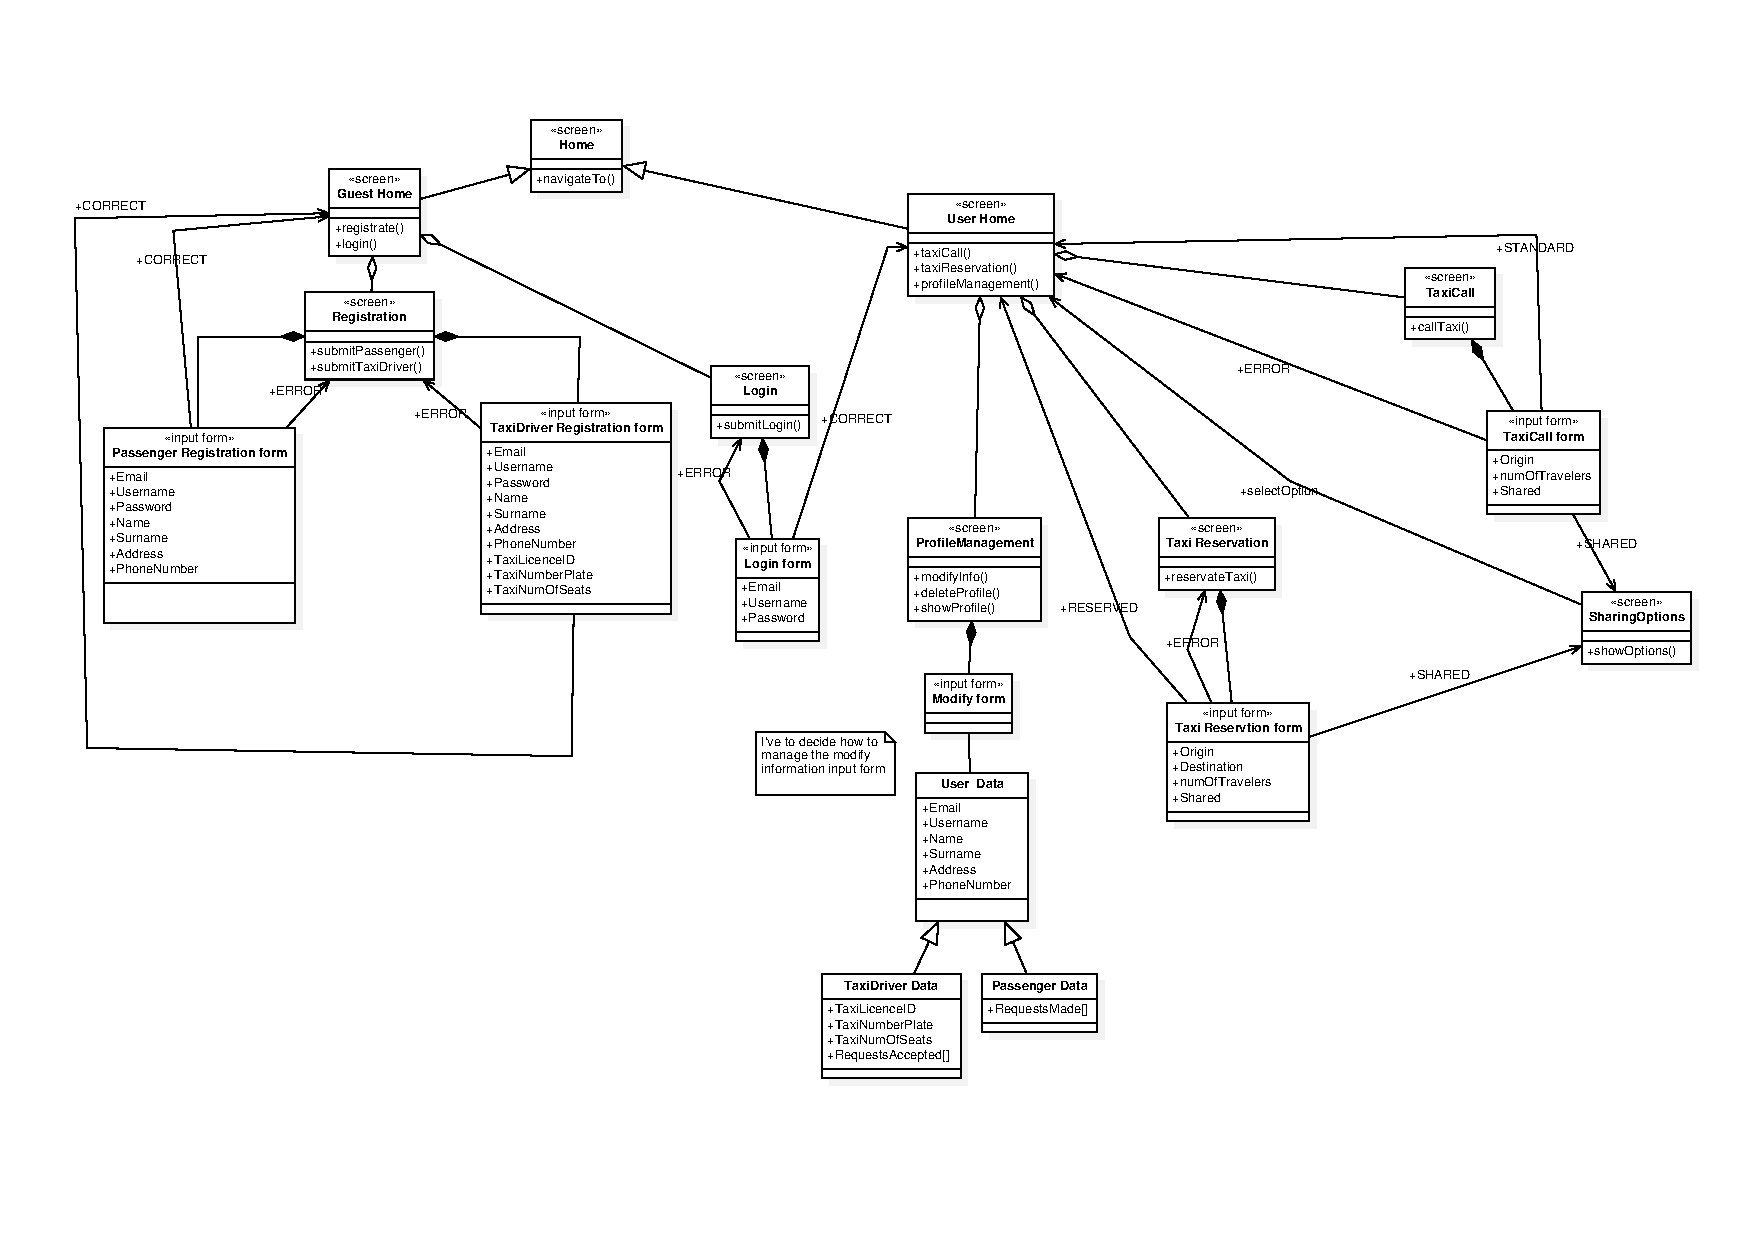
\includegraphics[width=\textwidth]{diagrams/UXdiagramSE2}
\caption{The UX diagram.}
\label{fig:ux-diagram}
\end{figure}

\FloatBarrier
\section{User Interface concept}

\subsection{Web interface}
These mock-ups show how the user interface for the web application should look like on web browser, also with the possibility to choose the language in every screen.

\begin{figure}[h]
\centering
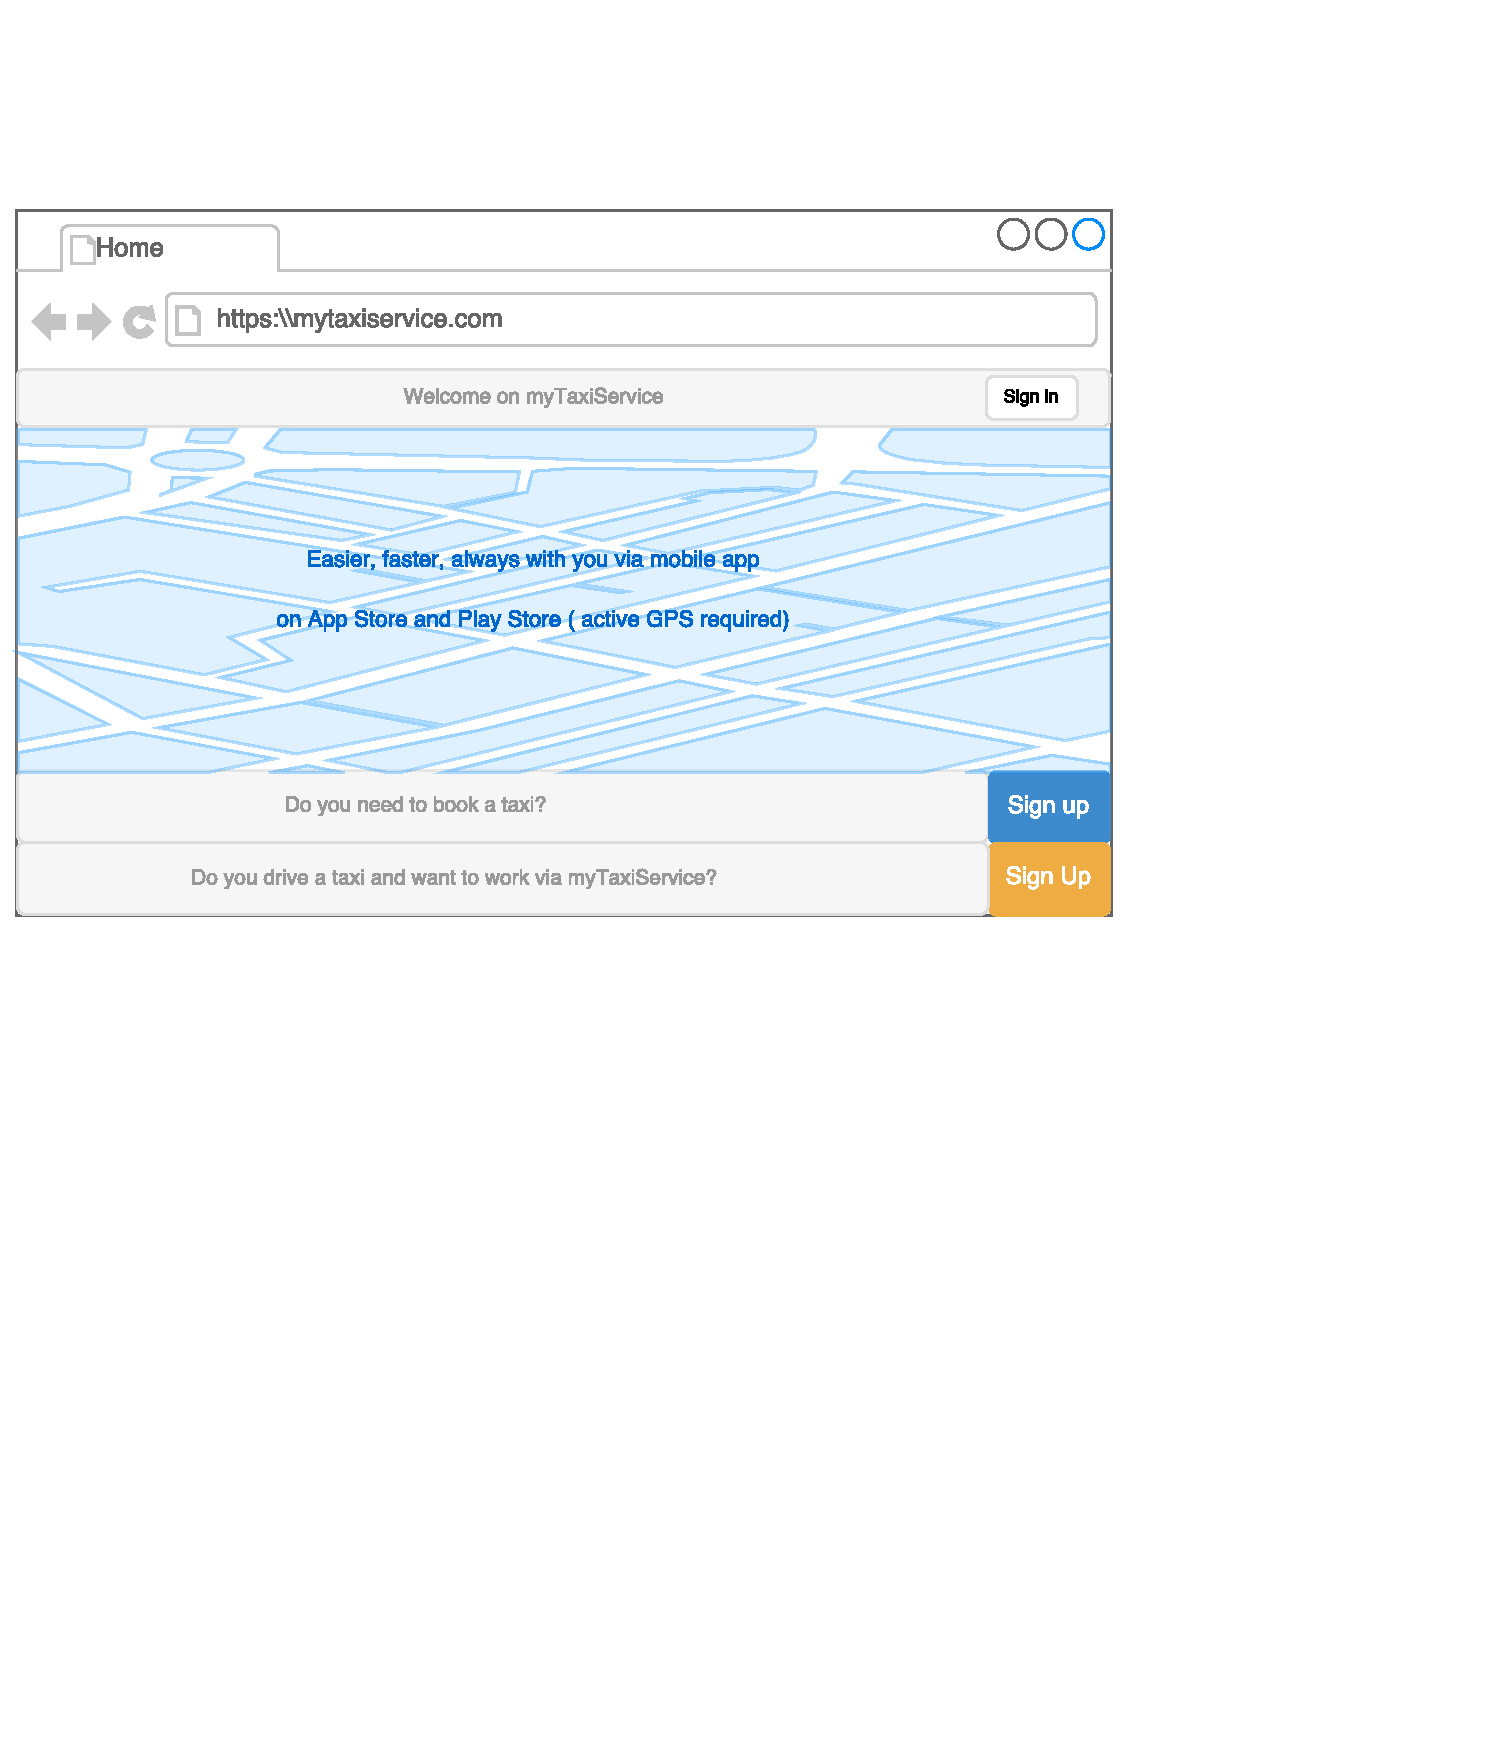
\includegraphics[width=0.7\textwidth]{mockup/web/GuestHome}
\caption{The home page of myTaxiService before log-in or registration.}
\label{fig:mockup-guesthome}
\end{figure}

\begin{figure}[h]
\centering
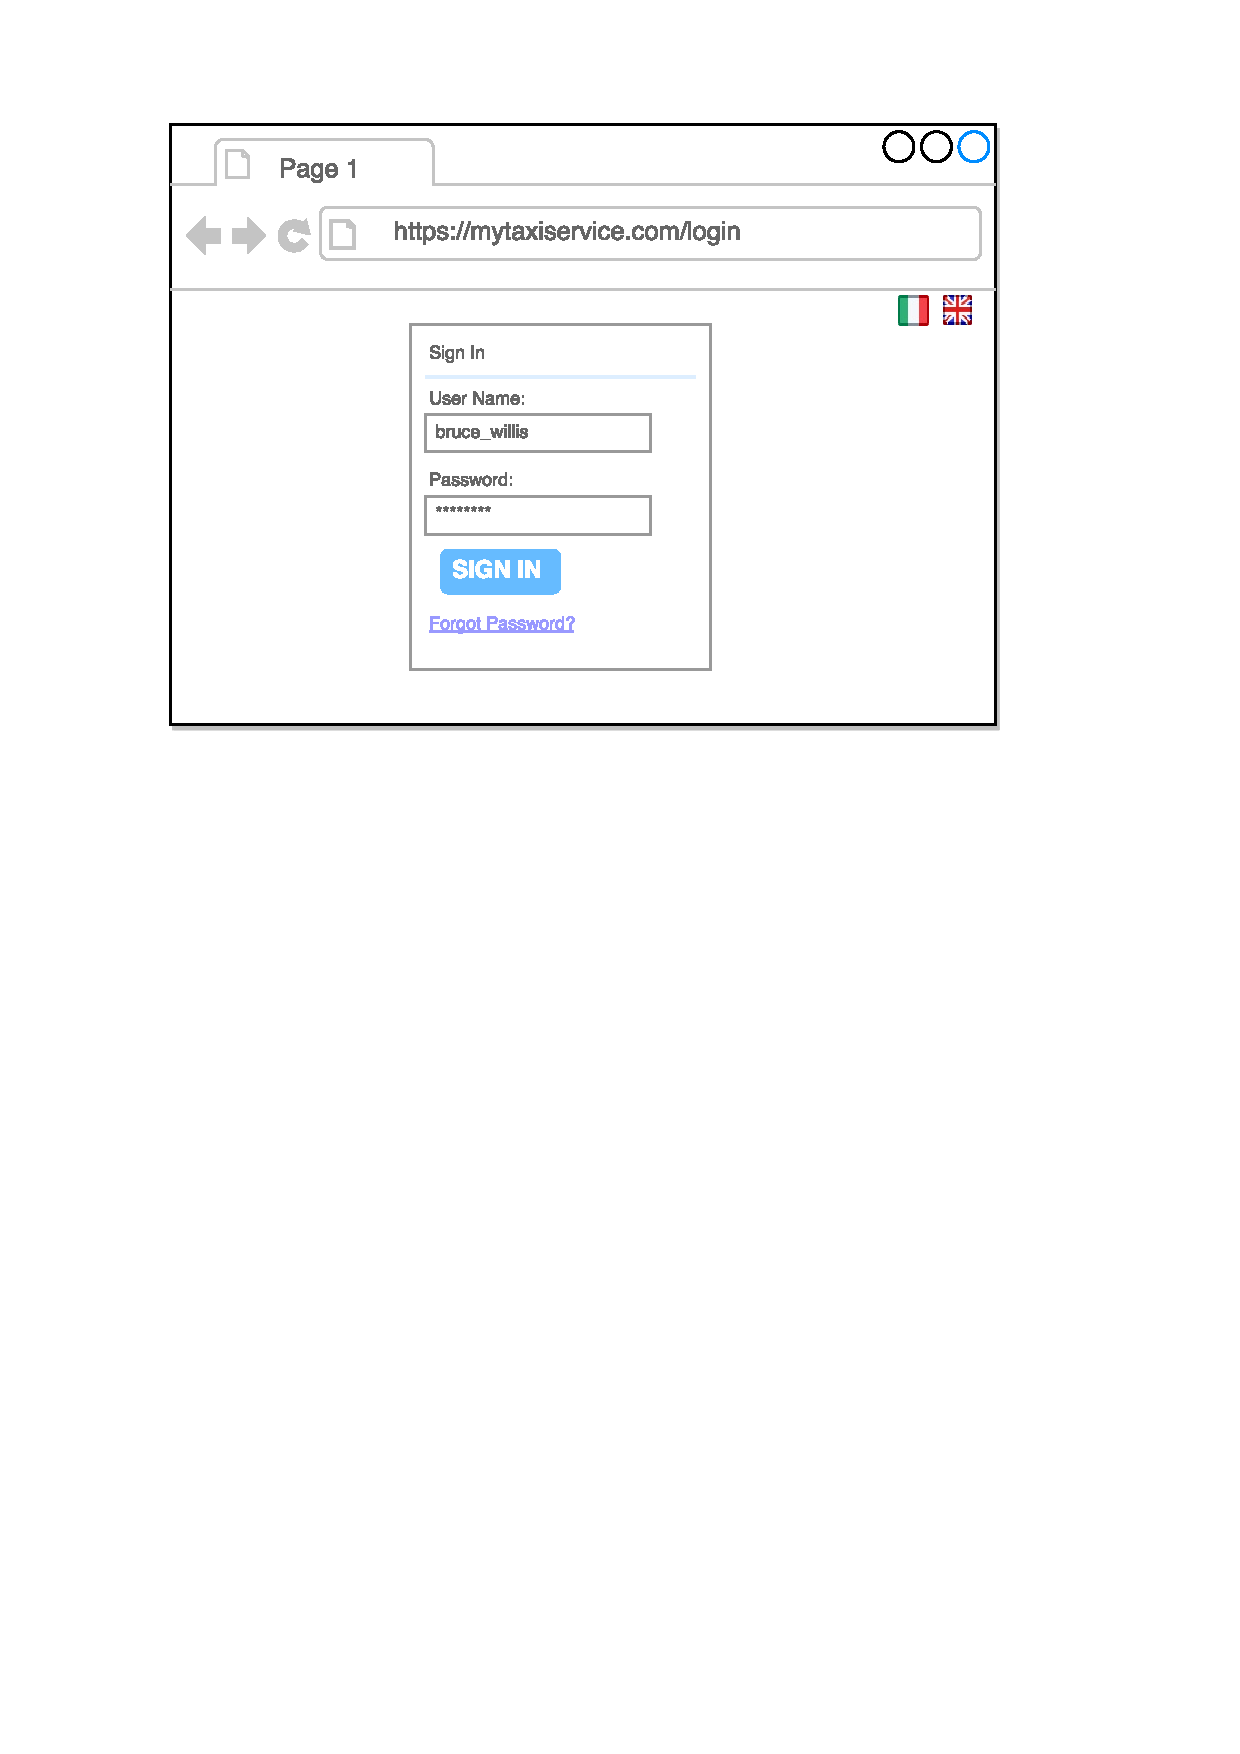
\includegraphics[width=0.7\textwidth]{mockup/web/Login_browser}
\caption{Login screen for the web application.}
\label{fig:mockup-login-browser}
\end{figure}

\begin{figure}[h]
\centering
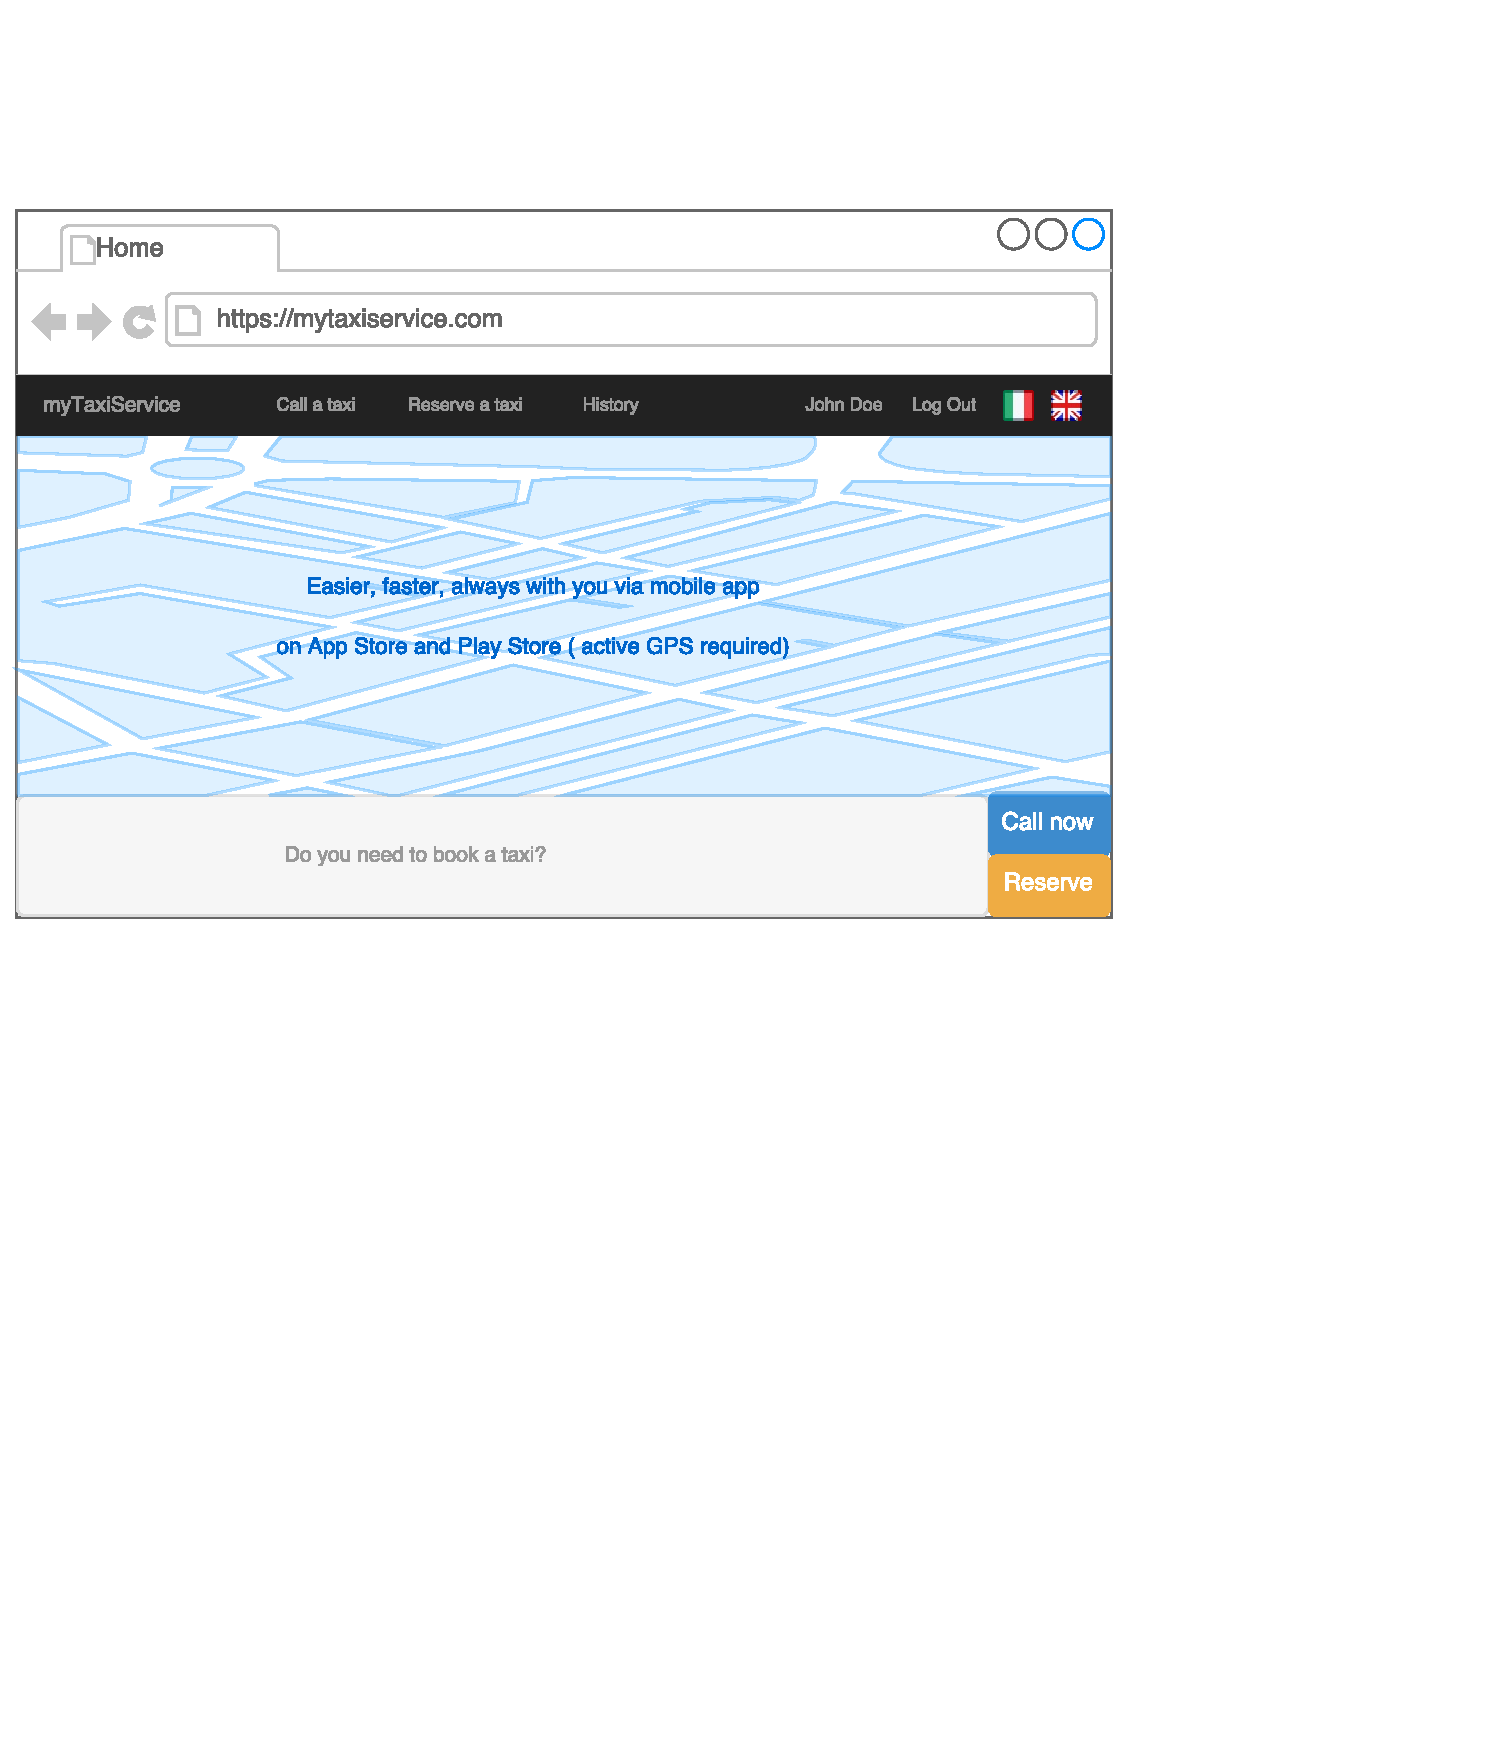
\includegraphics[width=0.8\textwidth]{mockup/web/UserHome}
\caption{Home page for the logged in passengers linking to all the functionalities.}
\label{fig:mockup-userhome}
\end{figure}

\begin{figure}[h]
\centering
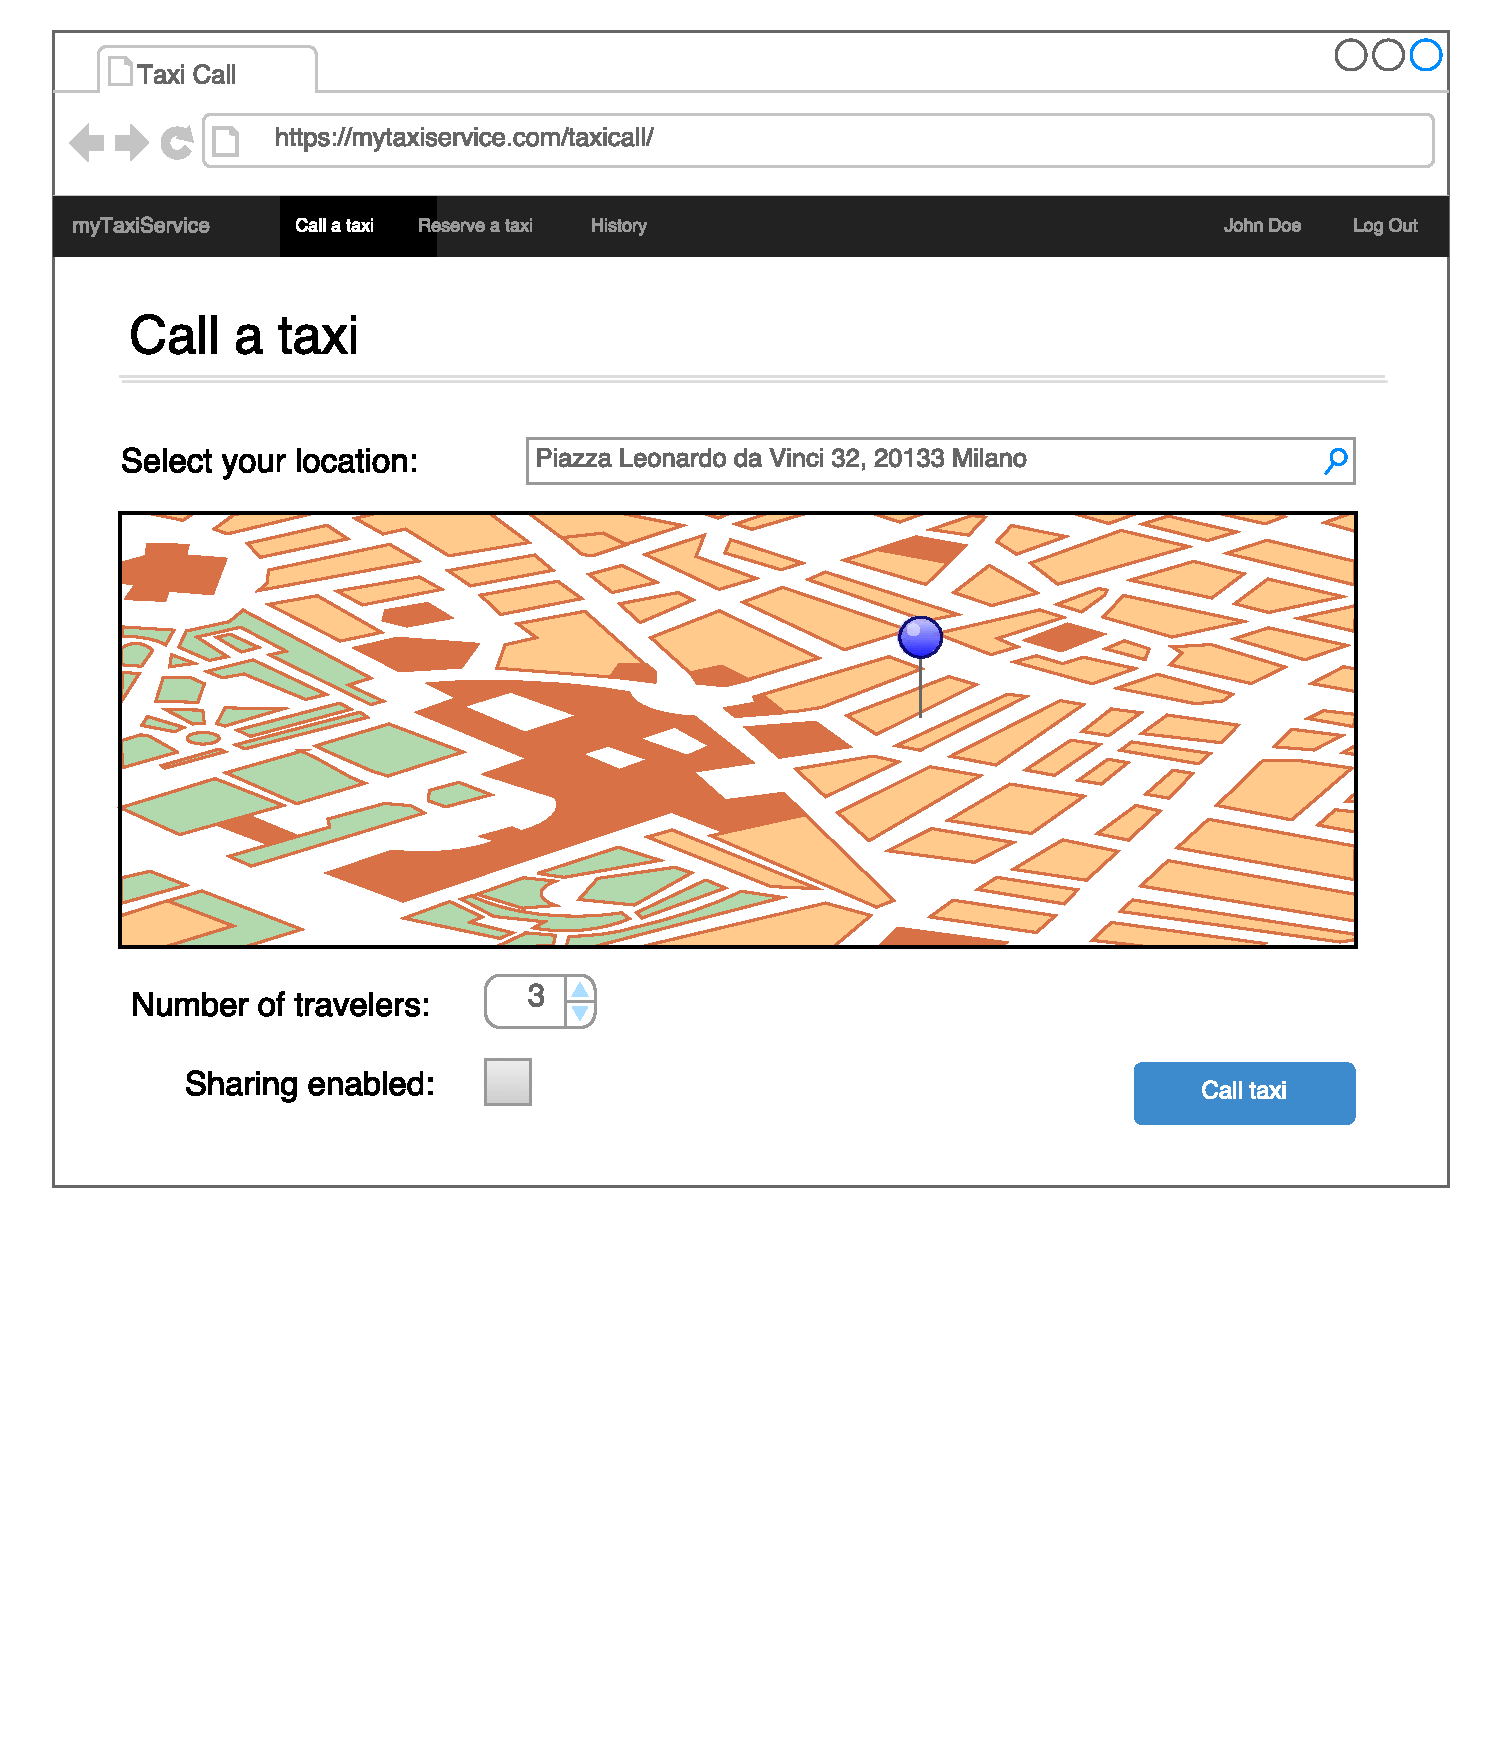
\includegraphics[width=0.8\textwidth]{mockup/web/TaxiCallBrowser}
\caption{Taxi call screen in the web application.}
\label{fig:mockup-taxicall-browser}
\end{figure}

\begin{figure}[h]
\centering
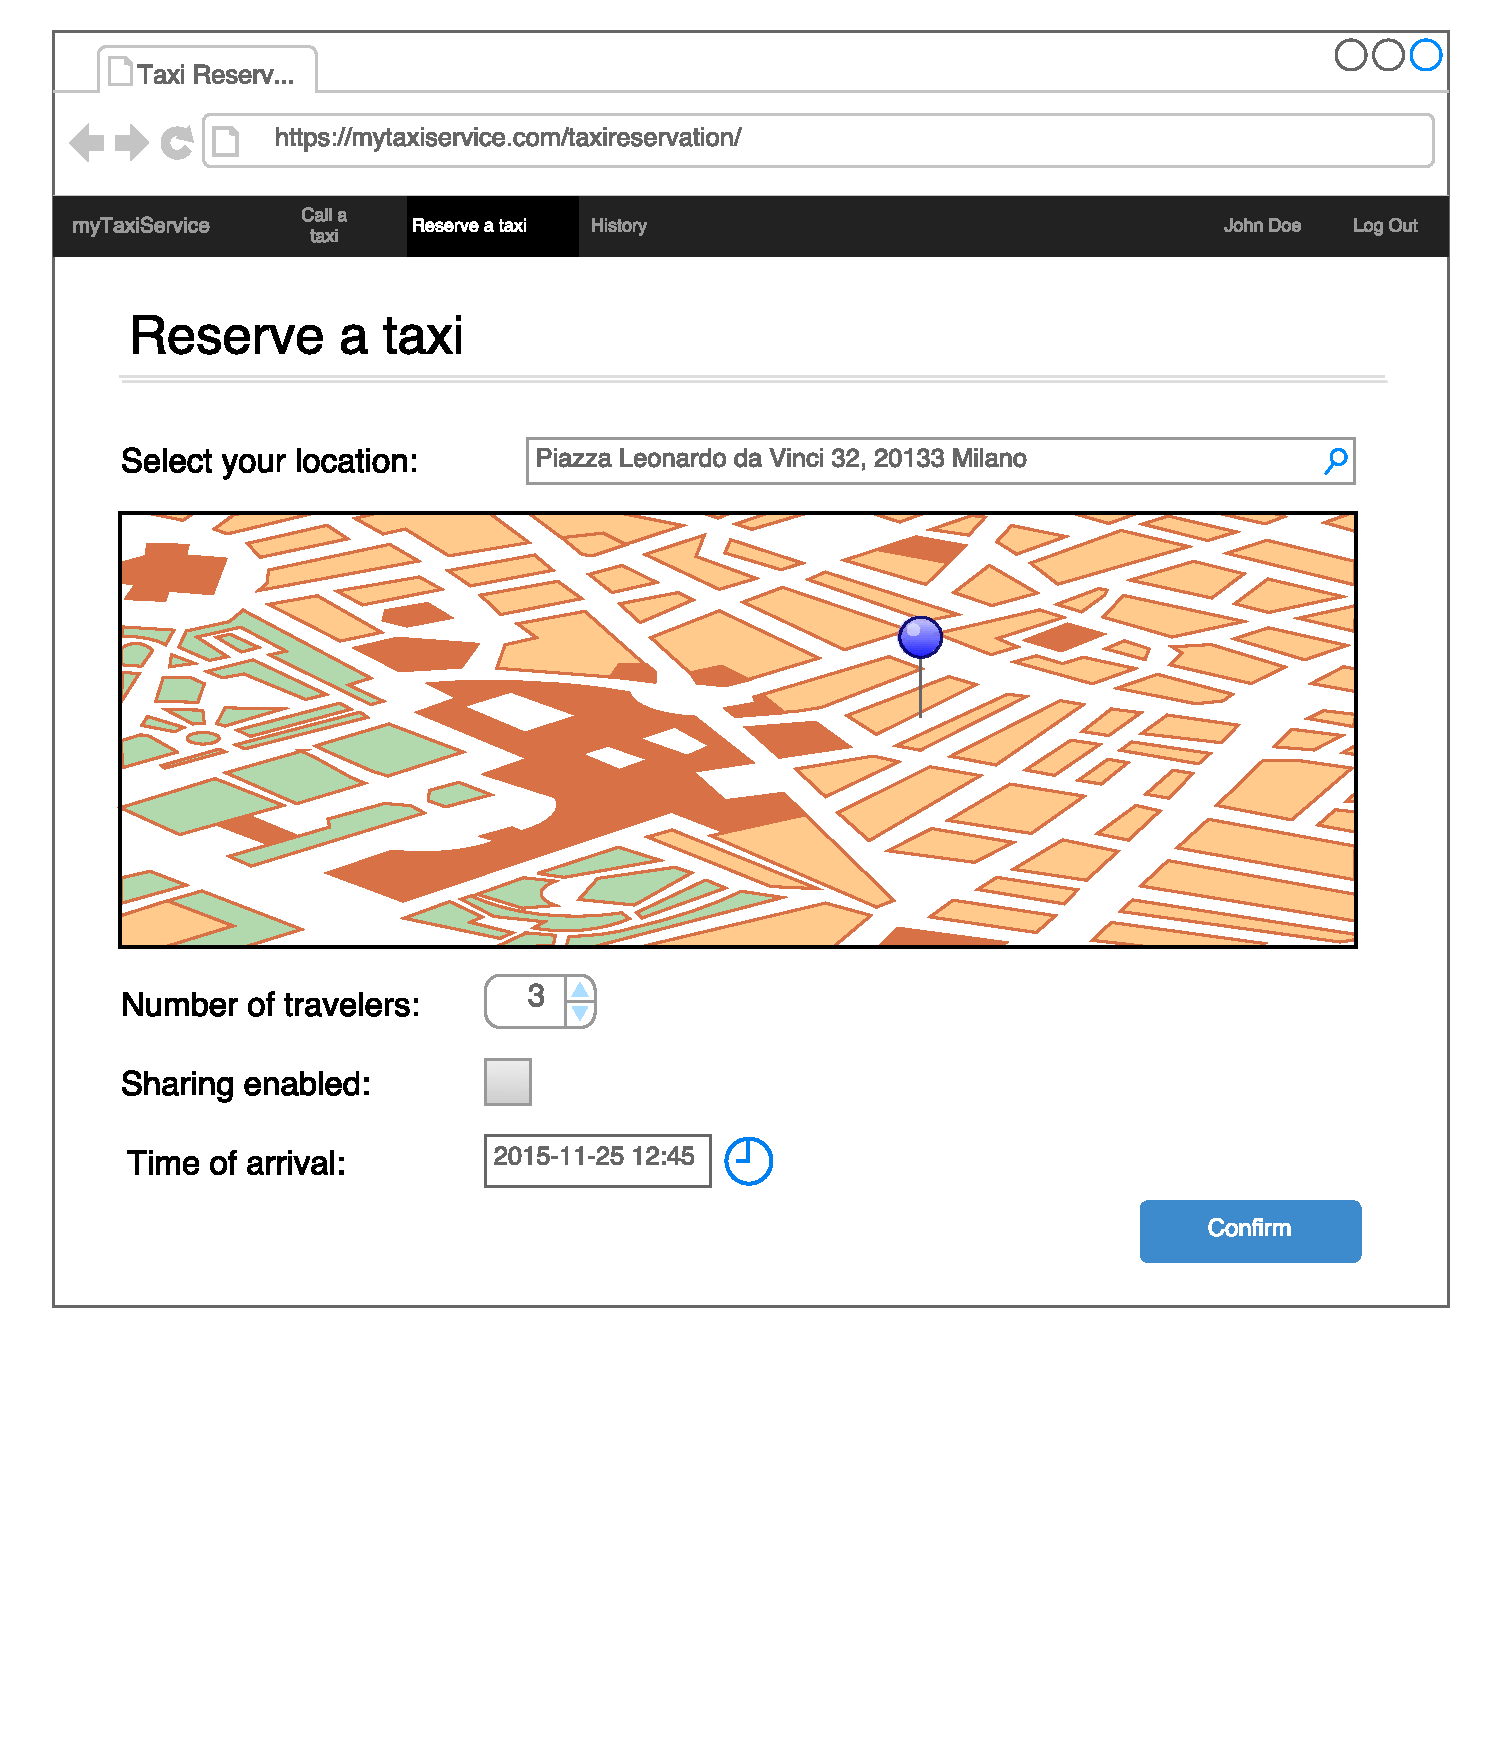
\includegraphics[width=0.8\textwidth]{mockup/web/TaxiReservationBrowser}
\caption{Taxi reservation screen in the web application.}
\label{fig:mockup-reservation-browser}
\end{figure}

\begin{figure}[h]
\centering
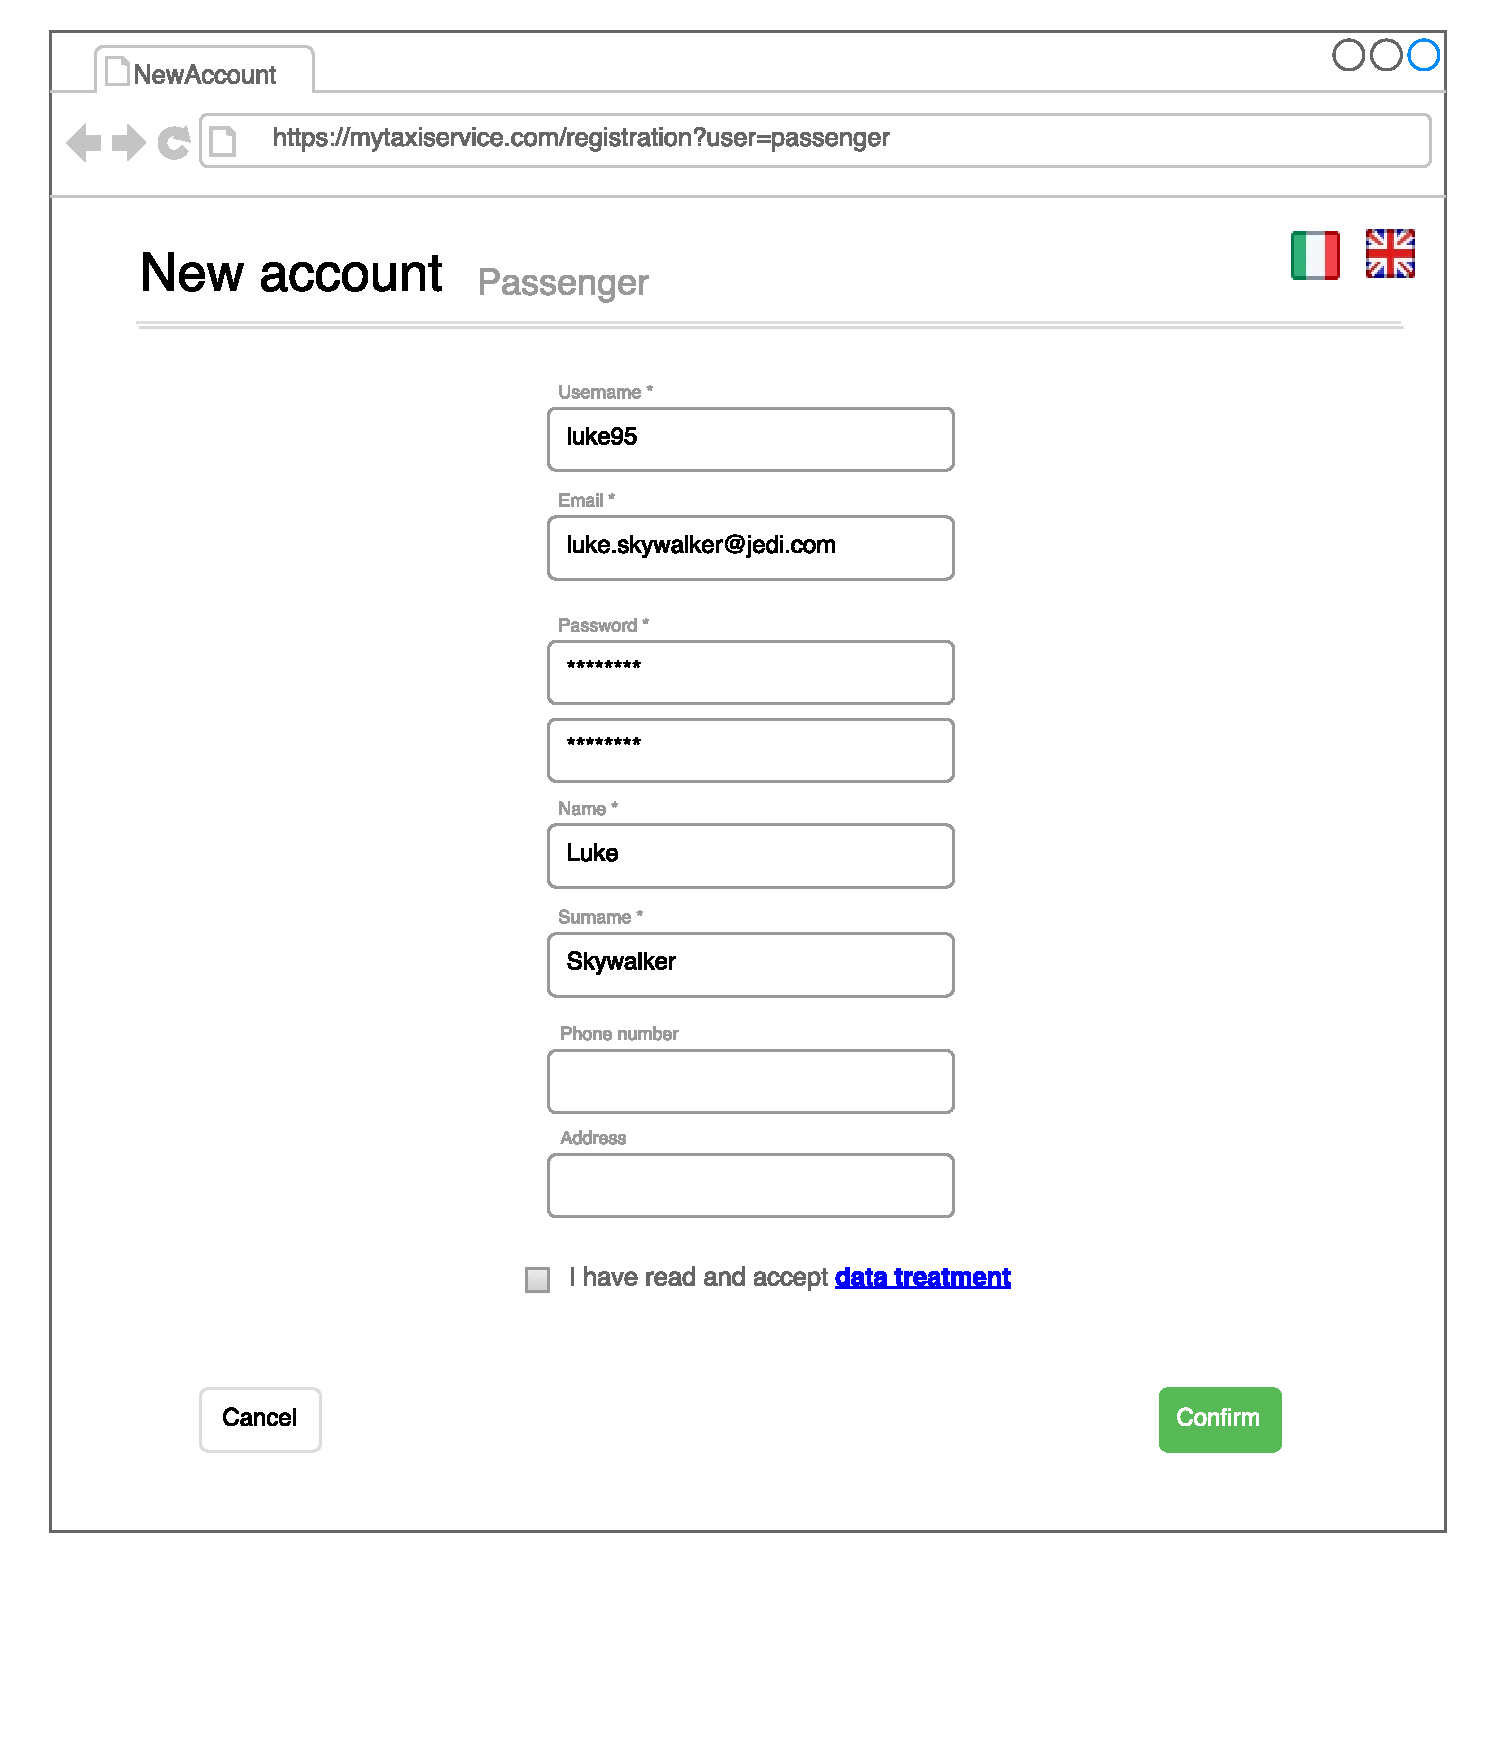
\includegraphics[width=0.9\textwidth]{mockup/web/Registration}
\caption{Registration screen for new users in the web application.}
\label{fig:mockup-registration}
\end{figure}

\FloatBarrier
\subsection{Mobile interface}
These mock-ups show how the interface of the myTaxiService mobile application will look like.

\begin{figure}[h]
    \centering
    \begin{subfigure}{0.45\textwidth}
        \centering
        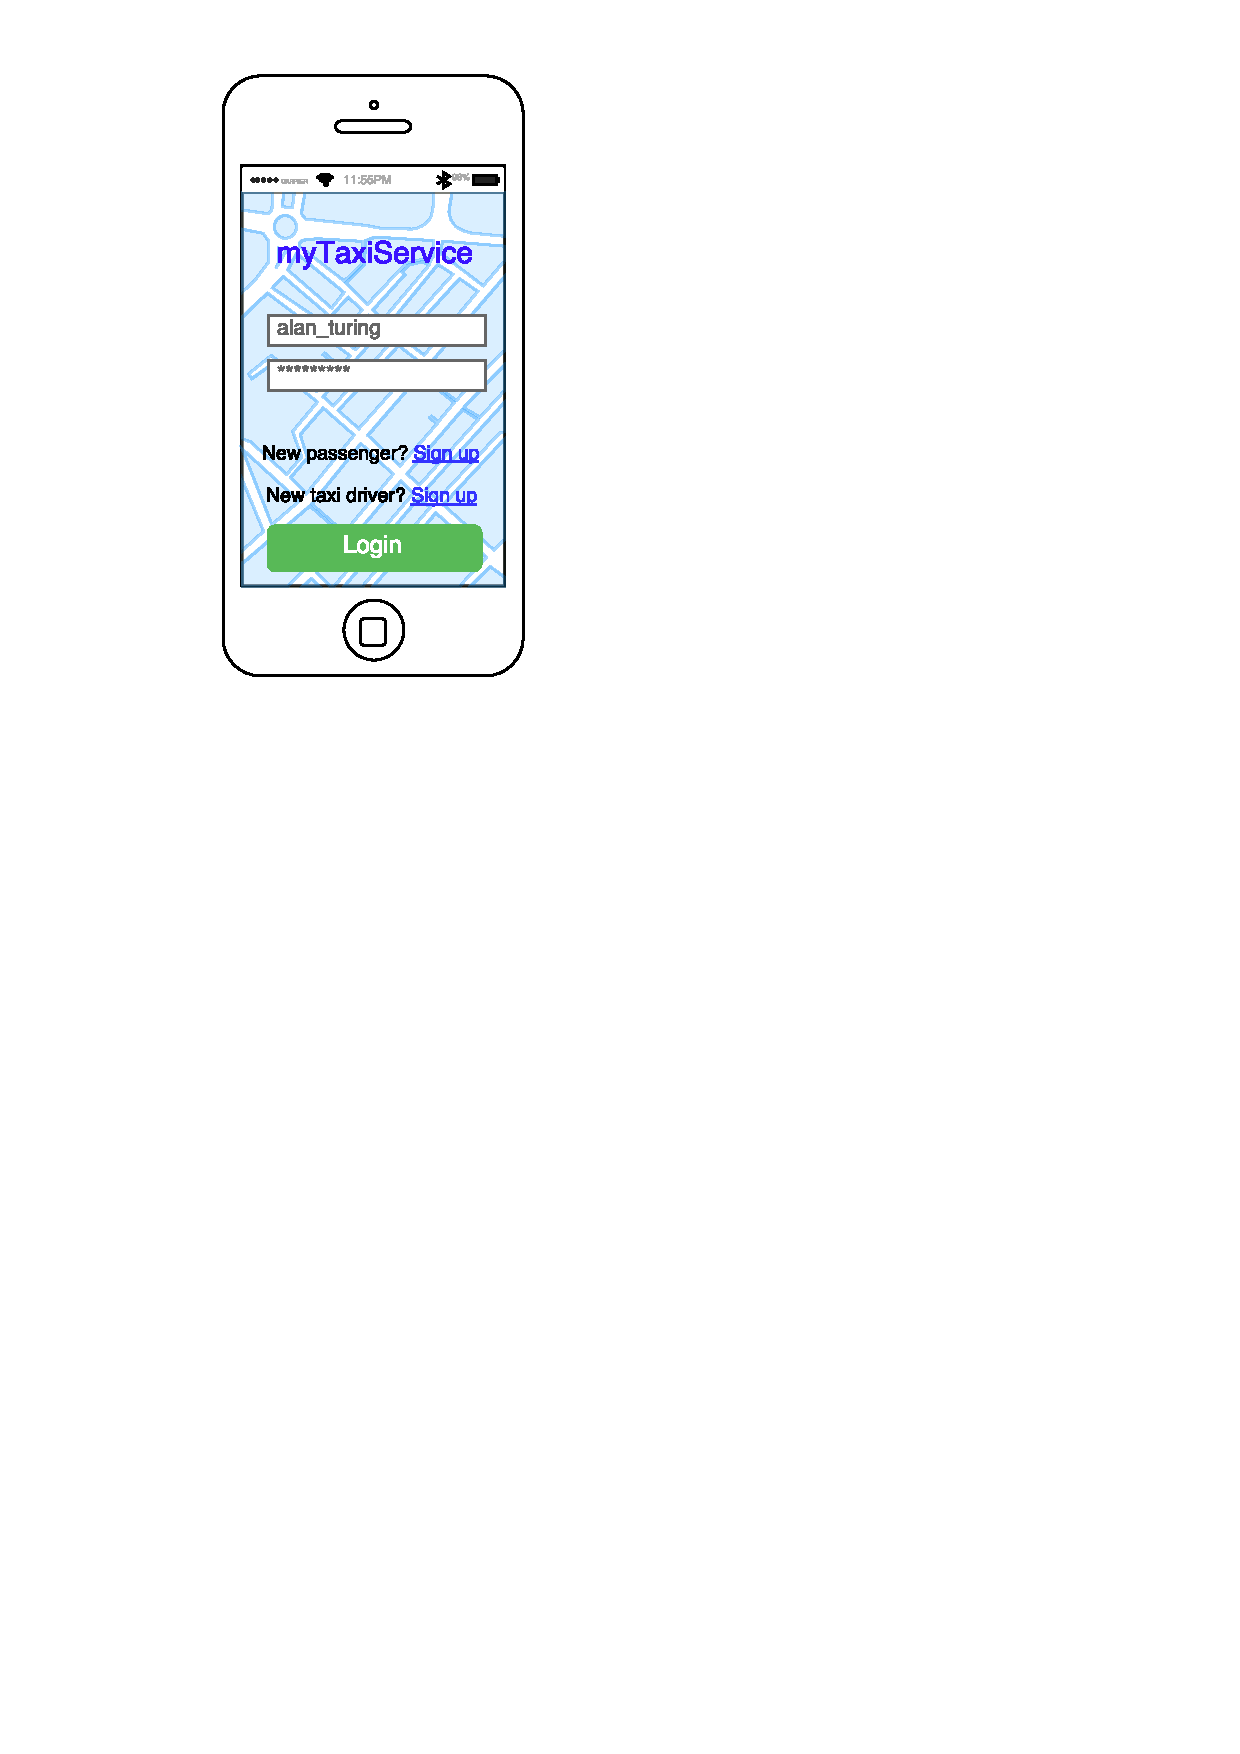
\includegraphics[width=\textwidth]{mockup/app/MobileLogin}
        \caption{Initial login screen on the mobile application. This screen also presents the option for signing up if the user does not have an account.}
        \label{fig:mockup-login-mobile}
    \end{subfigure}
    \hspace{1cm}
    \begin{subfigure}{0.45\textwidth}
        \centering
        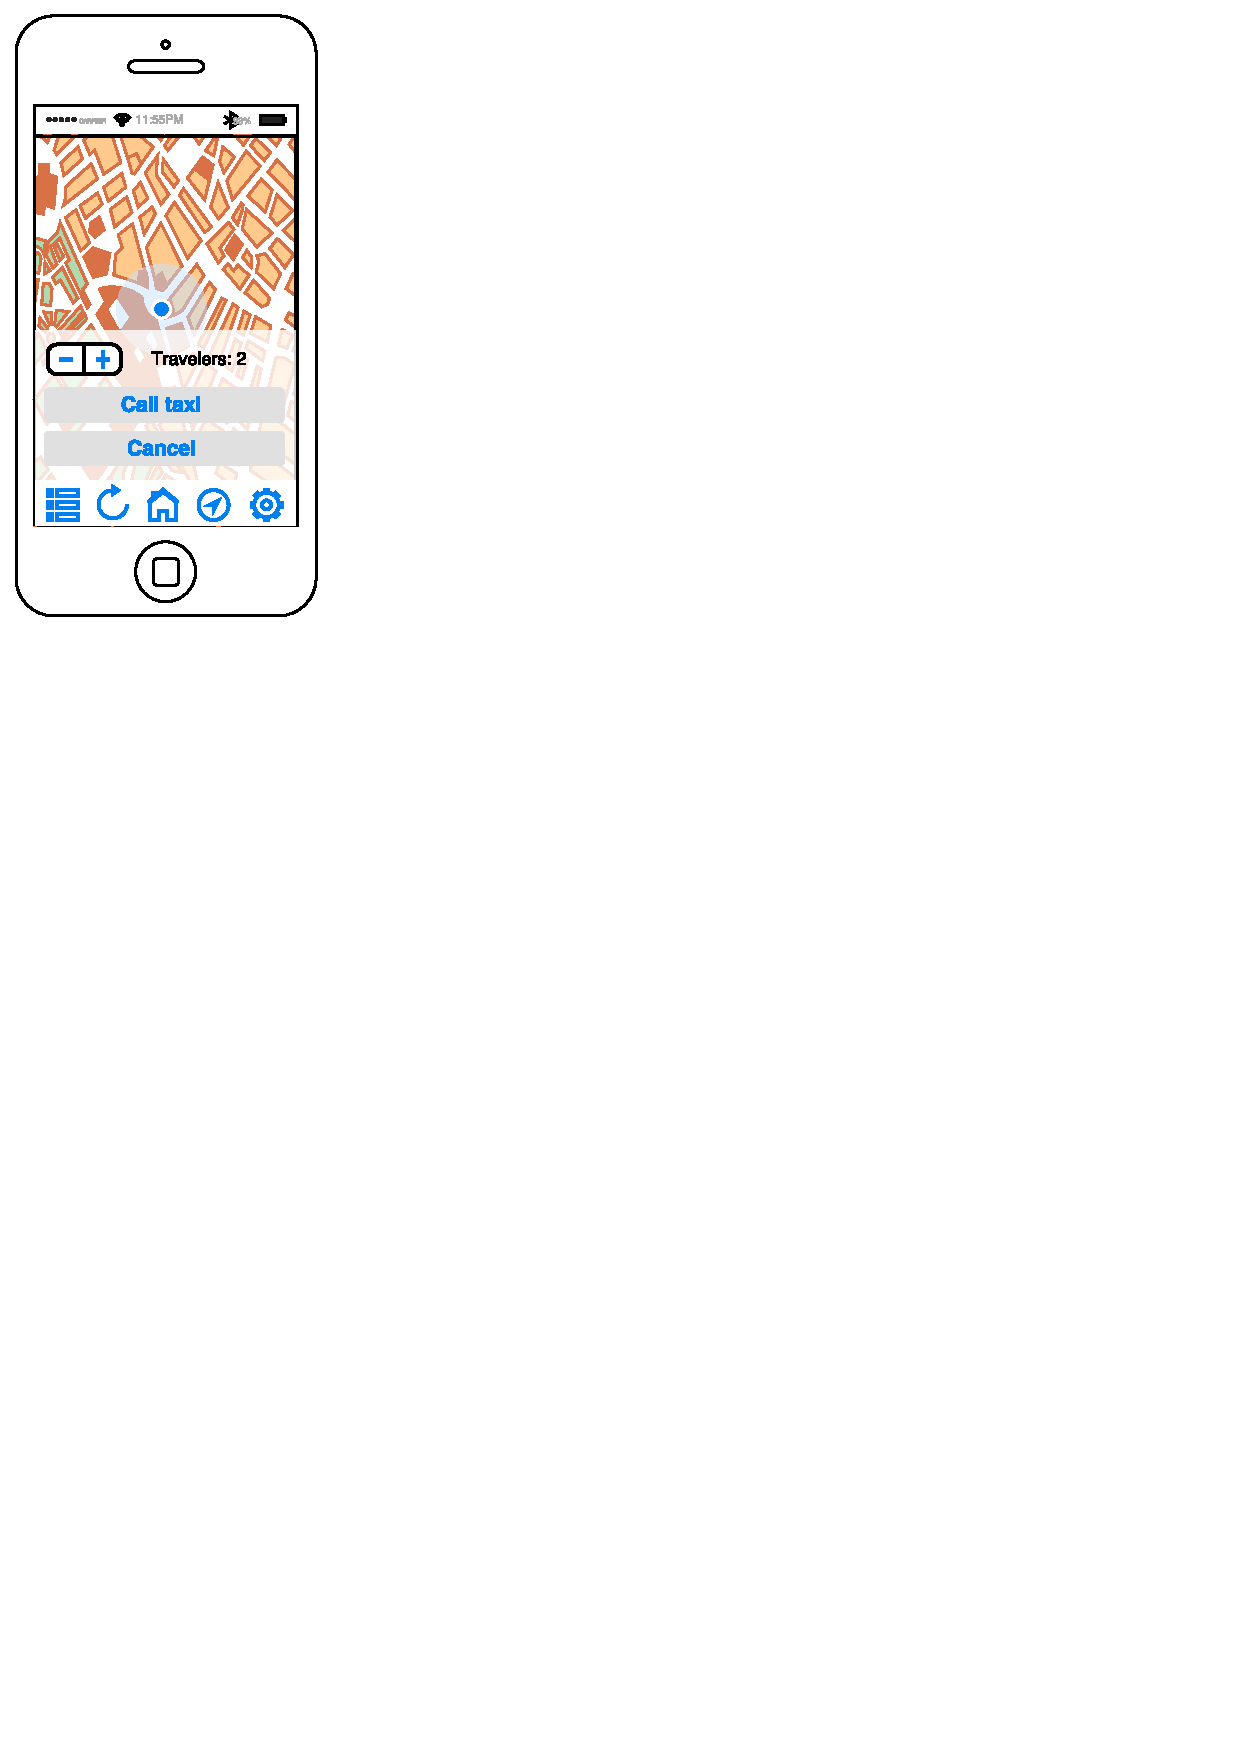
\includegraphics[width=\textwidth]{mockup/app/TaxiCall}
        \caption{Taxi call interface for the mobile application. The passenger may check if his location is correct and call a taxi specifying the number of travelers.}
        \label{fig:mockup-taxicall-mobile}
    \end{subfigure}
    \caption{Login and taxi call screens for the mobile application.}
\end{figure}

\begin{figure}[h]
    \centering
    \begin{subfigure}{0.45\textwidth}
        \centering
        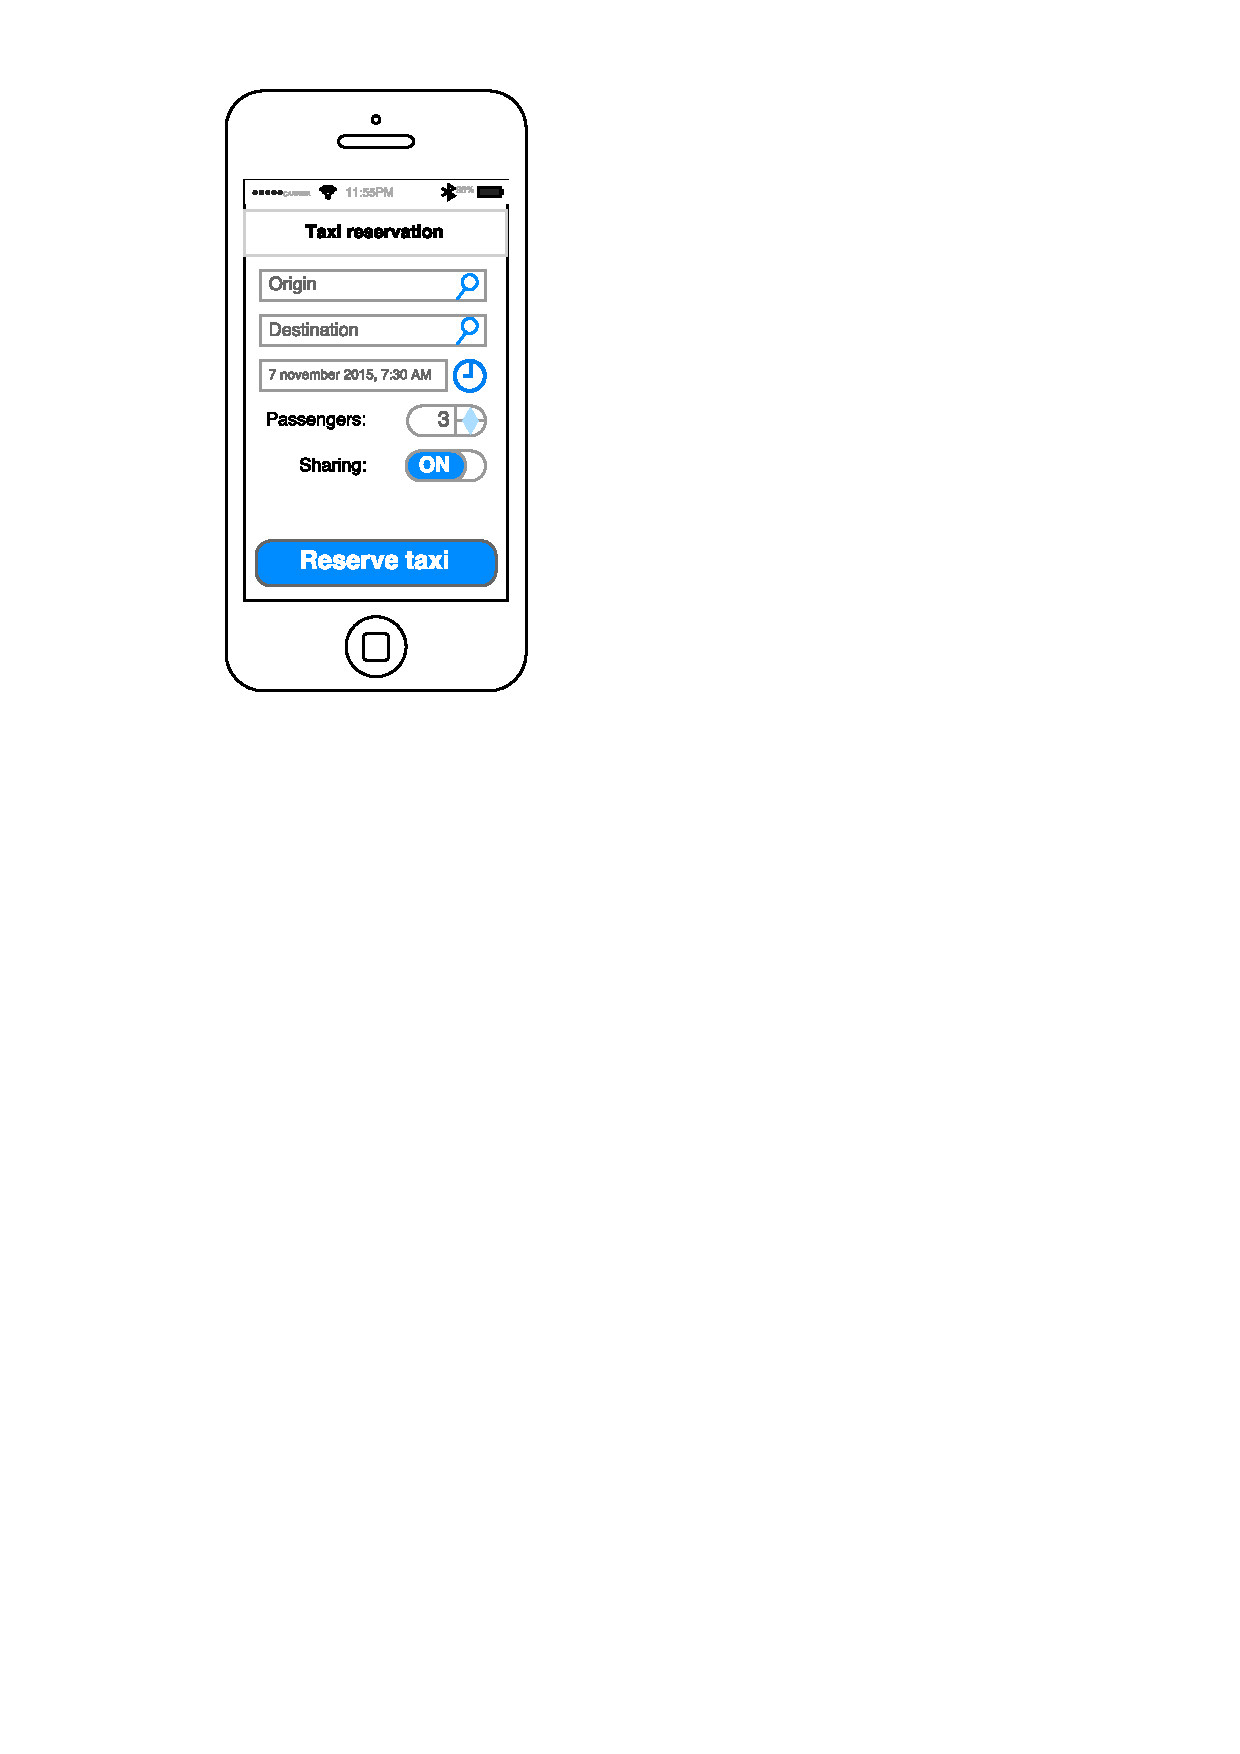
\includegraphics[width=\textwidth]{mockup/app/TaxiReservation}
        \caption{Taxi reservation screen for the mobile application.}
        \label{fig:mockup-reservation-mobile}
    \end{subfigure}
    \hspace{1cm}
    \begin{subfigure}{0.45\textwidth}
        \centering
        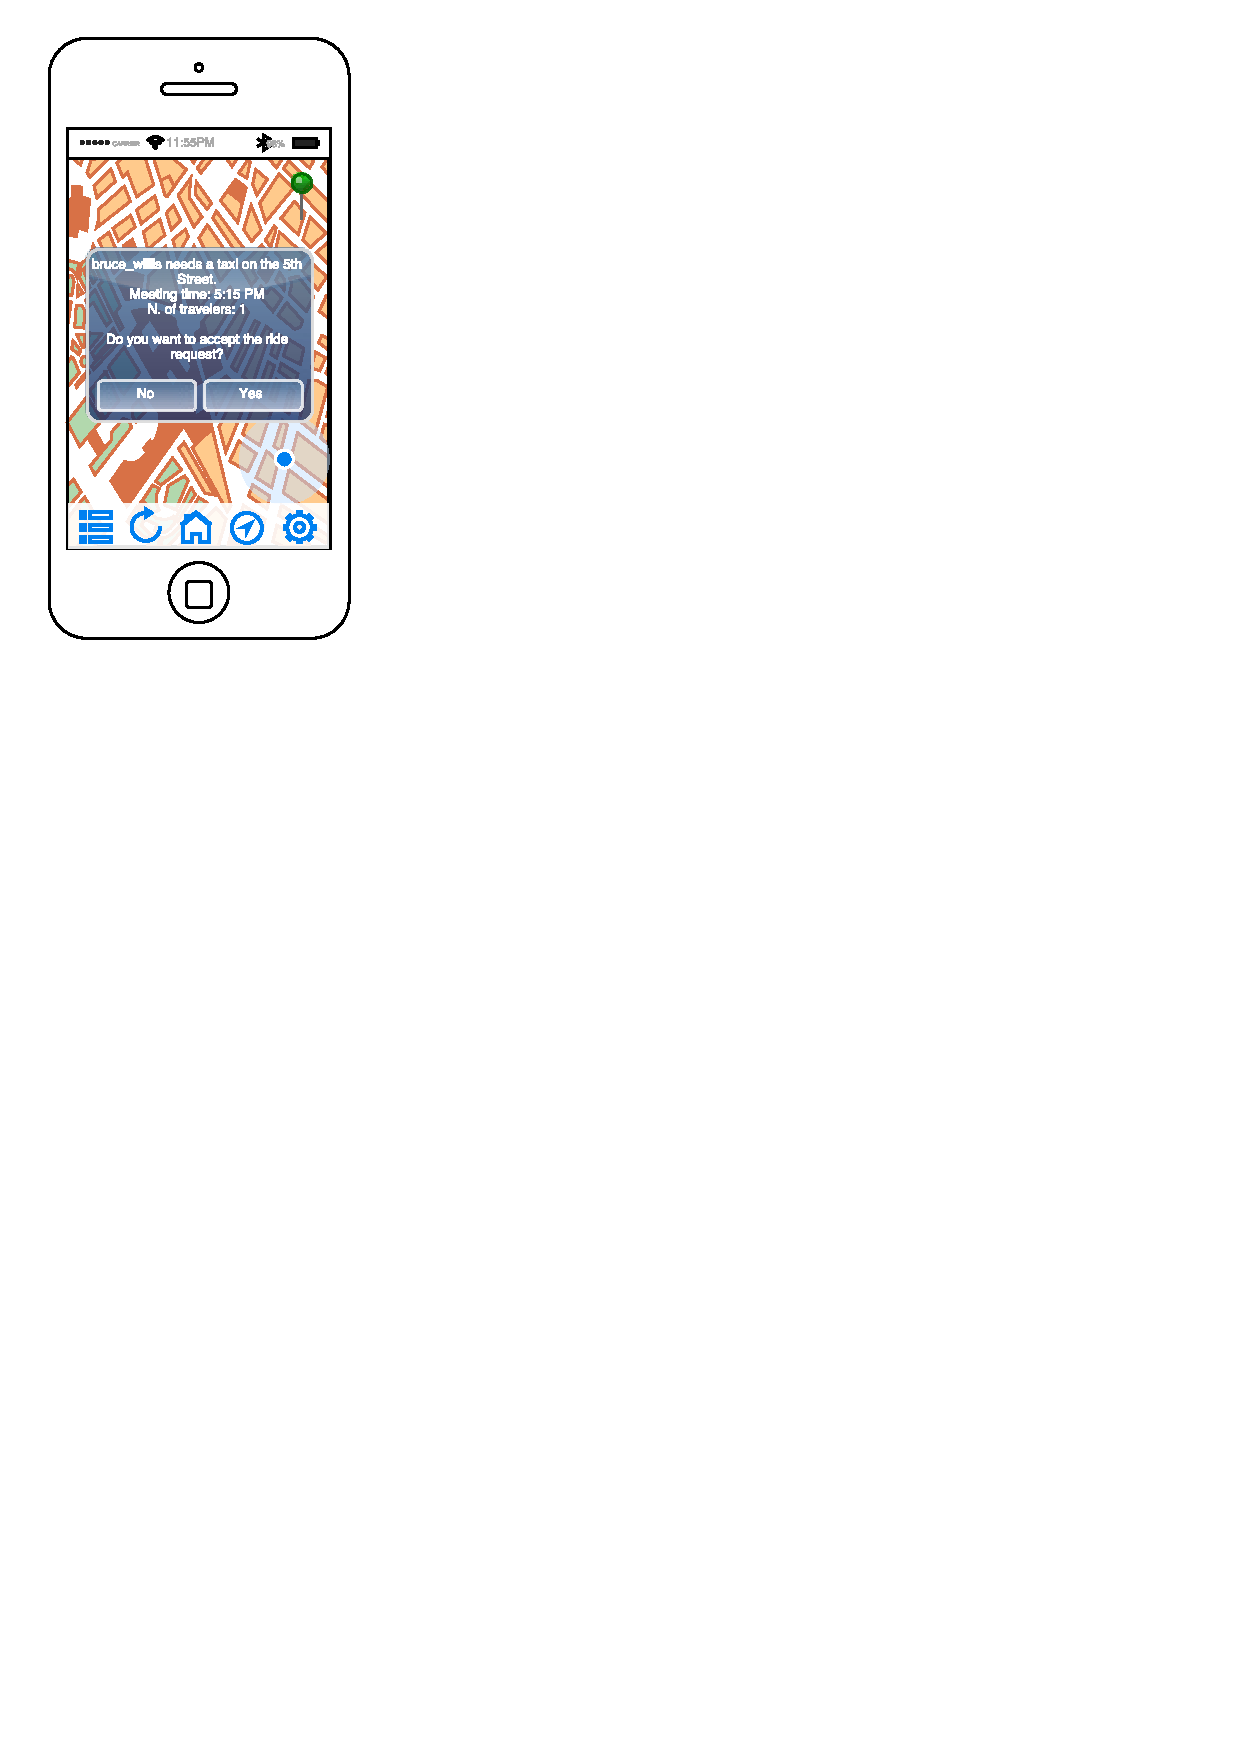
\includegraphics[width=\textwidth]{mockup/app/RideRequest}
        \caption{Ride request notification for taxi drivers in the mobile application.}
        \label{fig:mockup-riderequest-mobile}
    \end{subfigure}
    \caption{Taxi reservation and ride request screens for the mobile application.}
\end{figure}

%TODO Eleonora

% ------- REQUIREMENTS TRACEABILITY -------
\chapter{Requirements traceability}
\label{ch:requirements-traceability}

\appendix
\chapter{Appendix}

%% Settings for Alloy code listing.
\lstset{
    language=alloy,
    numbers=left,
    numberstyle=\tiny,
    stepnumber=2,
    tabsize=4,
    keywordstyle=\color{alloy-keyword}\bfseries,
    commentstyle=\color{alloy-comment},
    stringstyle=\color{alloy-string},
}

% Includes the Alloy model file.
\lstinputlisting{alloy/alloy_model.als}


\section{Software and tools used}
\begin{itemize}
    \item \LaTeX\, for typesetting this document.
    \item GitHub\footnote{\url{https://github.com}} for version control and distributed work.
    \item Draw.io\footnote{\url{https://www.draw.io/}} for mockups.
    \item StarUML\footnote{\url{http://staruml.io/}} for UML diagrams.
\end{itemize}

\section{Hours of work}
The statistics about commits and code contribution are available on GitHub~\footnote{\url{https://github.com/pietrodn/se2-mytaxiservice}}.
Please keep in mind that many commits are actually group work (when this is the case, it is stated in the commit message).

\begin{itemize}
    \item Eleonora Chitti: ?? hours
    \item Alex Delbono: 17 hours
    \item Pietro De Nicolao: 19 hours
\end{itemize}


\begin{thebibliography}{1}
\bibitem{w3c-html5}
  W3C,
  \emph{HTML5 - W3C Recommendation 28 October 2014}, \url{http://www.w3.org/TR/html5/}.

\bibitem{w3c-css}
  W3C,
  \emph{Cascading Style Sheets Level 2 Revision 1 (CSS 2.1) Specification}, \url{http://www.w3.org/TR/CSS21/}

\bibitem{apple-ios-hig}
	Apple,
	\emph{iOS Human Interface Guidelines}, \url{https://developer.apple.com/library/ios/documentation/UserExperience/Conceptual/MobileHIG/}
	
\bibitem{google-android-hig}
	Google,
	\emph{Android Developers - Design}
	\url{https://developer.android.com/design/index.html}
\end{thebibliography}

\end{document}
